 \documentclass[a4paper,11pt]{article}

\usepackage{amsmath}
\usepackage{amssymb}
\usepackage{amsthm}
\usepackage{graphicx}
\usepackage{caption}
\usepackage{subcaption}

\newtheorem{thm}{Theorem}
\newtheorem{lem}{Lemma}

\newcommand{\beq}{\begin{equation}}
\newcommand{\eeq}{\end{equation}}

\newcommand{\ba}{\begin{array}}
\newcommand{\ea}{\end{array}}

\newcommand{\bea}{\begin{eqnarray}}
\newcommand{\eea}{\end{eqnarray}}

\newcommand{\bc}{\begin{center}}
\newcommand{\ec}{\end{center}}

\newcommand{\ds}{\displaystyle}

\newcommand{\bt}{\begin{tabular}}
\newcommand{\et}{\end{tabular}}

\newcommand{\bi}{\begin{itemize}}
\newcommand{\ei}{\end{itemize}}

\newcommand{\bd}{\begin{description}}
\newcommand{\ed}{\end{description}}

\newcommand{\bp}{\begin{pmatrix}}
\newcommand{\ep}{\end{pmatrix}}

\newcommand{\p}{\partial}
\newcommand{\sech}{\mbox{sech}}

\newcommand{\cf}{{\it cf.}~}

\newcommand{\ltwo}{L_{2}(\mathbb{R}^{2})}
\newcommand{\smooth}{C^{\infty}_{0}(\mathbb{R}^{2})}

\newcommand{\br}{{\bf r}}
\newcommand{\bk}{{\bf k}}
\newcommand{\bv}{{\bf v}}

\setlength{\textheight}{212mm}
\setlength{\textwidth}{165mm}
\topmargin -6mm
\oddsidemargin -6mm


\newcommand{\gnorm}[1]{\left|\left| #1\right|\right|}
\newcommand{\ipro}[2]{\left<#1,#2 \right>}
\title{Vortex Patches under Cnoidal Waves}
\author{Christopher W. Curtis\\
Henrik Kalisch}
\date{}
\begin{document}
\maketitle
\section*{Abstract}

\section{Introduction}
The modeling of free-surface waves is a well studied and central area in several areas within applied mathematics, fluid mechanics, and oceanography.  Analytical concerns have motivated almost two-hundred years of work with a corresponding slew of techniques both formal and rigorous that have found use throughout applied mathematics; see \cite{constantin} and the historical notes contained therein.  The free-surface problem also appears as a fundamental problem in both old \cite{lamb} and modern \cite{kundu} classics on fluid mechanics. Perhaps the greatest role that the problem plays though is in formulating the foundation for spectral-wave modelling, which forms the core of much of modern data-driven oceanography \cite{holthuijsen}.

A long standing issue however in the modeling of free-surface waves is the impact that vorticity has on wave dynamics.  This has been considered an especially difficult problem for general vorticity profiles given that the momentum equation cannot be readily integrated up to the surface via the use of a harmonic potential.  Much progress has been made by making the simplifying assumption of the vorticity being a constant leading to seminal numerical and analytic studies of these problems, see \cite{constantin,pullin1,simmen,dasilva} among many others.  In a similar vein, one can see the stability theory of shear profiles \cite{craik2,craik3,drazen,phillips1} as another means of addressing the impact of vorticity on free surface flows.  This approach has been pushed to higher order, nonlinear models with corresponding numerical implementations in \cite{nwogu2}.

However, in neither case can one track the evolution of an arbitrary vortex profile.  As shown in experiment \cite{liu1,liu2,lin}, the motion of solitary waves over bathymetric features induces the formation of vortex patches.  Likewise, it is clear that accurate near shore modeling involves an understanding of the fluid vorticity profile and its interactions with the free surface.  Progress in this direction has been made by assuming shallow-water scalings and deriving various Boussinesq-like models \cite{nwogu1,chen,zhang} or Green-Naghdi models \cite{Lannes2014_1,Lannes2014_2,Lannes2016_1}.  These approaches, while limited to near-shore conditions, allow markedly enhanced modeling of shoaling and can be coupled to phenomenological models of wave-breaking induced turbulence to allow for very accurate near-shore computation.  

In contrast to the above work, a body of numerical methods has developed within computational fluid mechanics known as Point-Vortex Methods (PVMs).  These are numerical schemes which track the evolution of compactly supported vorticity profiles via direct discretizations of the vorticity profile; see \cite{cottet,koumoutsakos,koumoutsakos2,krasny,beale,majda} among several others.  These schemes are especially attractive in that they do not place any strong restrictions on the flow and are suitable for simulations across a wide range of scales and geometries \cite{koumoutsakos3,koumoutsakos4}.  It was then shown in \cite{curtis} that, by incorporating the methodology for reformulating the free-surface problem as found in \cite{afm}, that PVMs could be in effect merged with Dirichlet-to-Neumann Operator (DNO) based methods \cite{craig,guyenne} for solving the free surface problem.  While requiring periodic boundary conditions, the approach in this paper allows for arbitrary depth and modeling accuracy, thus providing a distinct complement to the Boussinesq and Green-Naghdi models described above.

However, in \cite{curtis}, simulations with at most four vortices were studied, preventing the modeling of more complicated vortex patches underneath free surface waves.  Thus, in this paper we present simulations of vortex patches involving several thousands of vortices.  To do so, we incoporate into the formulation in \cite{curtis} many of the techniques for error control and computational efficiency that have been developed in the PVMs community.  In particular the use of a Fast-Multipole Method \cite{greengard} and Lagrangian-to Eularian regridding \cite{koumoutsakos} play critical roles in obtaining our results.  Using this machinery, by moving to shallow-water scalings, we are able to then study the impact of vortex patches on the evolution of free surfaces waves which are approximated by the cnoidal-solutions of the Korteweg--de Vries equation.  This is a canonical model for nonlinear, shallow-water free surface waves, and it thus serves as an excellent source for the generation of families of initial conditions for the free-surface state.  

As we show, vortex patches can induce nontrivial deformations of a free surface wave.  This deformation is more pronounced the more linear the surface wave is, or the better a small amplitude modal approximation is to the free surface.  This can best be understood by examing the relative input of energy into the free surface.  As shown, the less nonlinear the surface wave, the more energy it receives from the vortex patch, thereby creating high-frequency oscillations and thus significant distortions of the wave profile.  Likewise, we see that the transport of the patch itself is significantly enhanced when larger amplitude nonlinear surface waves move over the patch, which pulls energy from the surface to increase its speed of propagation.  The surface wav      

An overview of the paper is as follows.  In Section 2, the model, numerical scheme, and implementation details are presented.  Section 3 presents our numerical results, while in Section 4 we summarize our results and speak to future directions.  An Appendix collects technical details about the DNO.  
%%%%%%%%%%%%%%%%%%%%%%%%%%%%%%%%%%%%%%%%%%%%%%%%%%%%%%%%%%%%%%%%%%%%%%%%%%%%%%%%%%%
\section{Model, Numerical Scheme, and Implementation Details}
Throughout, we are attempting to describe the simultaneous evolution of a free surface $y = \eta(x,t) + H$, and a compactly supported patch of vorticity $\omega(x,y,t)$ underneath the free surface.  We suppose along the curve $z=0$ that we have a solid boundary so that the normal velocity is identically zero.  In an inviscid, incompressible fluid, we can represent the fluid velocity ${\bf u}(x,y,t)$ generated by a vortex patch characterized by vorticity profile $\omega({\bf x},t)$, ${\bf x}=(x,y)$, over the compact domain $\Omega(t)$ via the integral equation
\[
{\bf u}({\bf x},t) = \int_{\Omega(t)} {\bf K}({\bf x}-\tilde{{\bf x}})\omega(\tilde{{\bf x}},t)d\tilde{{\bf x}} + \nabla \tilde{\phi}, ~ \Delta \tilde{\phi} = 0.
\]
where $\omega$ is the vorticity, and ${\bf K}$ is the standard Biot-Savart kernel.  The harmonic function $\tilde{\phi}$ is used to address boundary conditions as explained in \cite{saffman}.  An attractive means for discretizing this equation as summarized in \cite{cottet} is to approximate the vorticity $\omega$ via the expression $\omega_{d}$ which is given by a collection of $N$ point-vortices at positions ${\bf x}_{j}(t)$ via the PVM expansion
\begin{equation}
\omega_{d}(\tilde{{\bf x}},t) = \sum_{j=1}^{N} \frac{\Gamma_{j}}{\delta^{2}}\chi\left(\frac{\tilde{{\bf x}}-{\bf x}_{j}(t)}{\delta}\right), ~ {\bf x}_{j}(t) = \left(x_{j}(t),y_{j}(t) \right),
\label{discvort} 
\end{equation}
where $\chi$ is some appropriately chosen mollifier, see \cite{beale}, and $\Gamma_{j}$ is the circulation associated with the point vortex at ${\bf x}_{j}(t)$.  Thus, we can reduce the problem of tracking the evolution of the vortex patch to describing the motion of the point vortices via the system of ODE's
\[
\frac{d{\bf x}_{j}}{dt}  =  \sum_{l\neq j}^{N} \Gamma_{l} {\bf K}_{\delta}\left({\bf x}_{j}-{\bf x}_{l}\right) + \nabla \tilde{\phi}\left({\bf x}_{j},t\right), ~ {\bf K}_{\delta}({\bf x}) = \frac{1}{\delta^{2}}\int_{\mathbb{R}^{2}}{\bf K}({\bf x} - \tilde{\bf x})\chi \left(\frac{\tilde{{\bf x}}}{\delta} \right) d \tilde{{\bf x}}.
\]
Choosing, as in \cite{beale}, the mollifier $\chi$ to be the fourth-order kernel 
\[
\chi(r) = 2e^{-r^{2}} - \frac{1}{2}e^{-r^2/2}, 
\]
introducing periodic boundary conditions in the lateral direction and enforcing the presence of a solid boundary along the curve $z=0$ then modifies the above dynamical system to be 
\[
i\frac{d z^{\ast}_{j}}{dt}  = \frac{1}{2\pi}\left(\sum_{l\neq j}^{N} \Gamma_{l} \sum_{m=-\infty}^{\infty} \frac{\tilde{\chi}(z_{j}-z_{l}-2Lm;\delta)}{z_{j}-z_{l}-2Lm} -   \sum_{l=1}^{N} \Gamma_{l} \sum_{m=-\infty}^{\infty} \frac{\tilde{\chi}(z_{j}-z^{\ast}_{l}-2Lm;\delta)}{z_{j}-z^{\ast}_{l}-2Lm}\right)  + \p_{y}\tilde{\phi} + i\p_{x}\tilde{\phi}, 
\]
where $z_{j}=x_{j} + iy_{j}$, the period in $x$ is given by $2L$, and
\[
\tilde{\chi}(r;\delta) = \left(1-e^{-r^{2}/2\delta^{2}} \right)\left(1+2e^{-r^{2}/2\delta^{2}} \right).
\]
We evalute the corresponding sums over the image points $z_{j}-z_{l}^{\ast}$ so as to keep the zero flow through $z=0$ condition strictly enforced.  

Following the arguments in \cite{curtis}, and again emphasizing the compact support of the vorticity $\omega(x,y,t)$, we then have at the free surface the coupled nonlinear system
\[
\p_{t}\eta = -\p_{x}\eta\p_{x}\tilde{\phi} + \p_{z}\tilde{\phi} + P_{v},
\]
and
\begin{multline*}
\p_{t}\tilde{\phi} + \frac{1}{2}\left|\nabla \tilde{\phi}\right|^{2} +\mbox{Im}\left\{Q_{v}\right\}\p_{x}\tilde{\phi} + \mbox{Re}\left\{Q_{v}\right\}\p_{z}\tilde{\phi} + g\eta = E_{v} - \frac{1}{2}\left|Q_{v}\right|^{2} + \frac{\sigma}{\rho_{0}}\p_{x}\left(\frac{\p_{x}\eta}{\sqrt{1+(\p_{x}\eta)^{2}}} \right)
\end{multline*}
where we have defined
\[
c(\eta,z_{j}) = \cot\left(\frac{\pi}{2L}\left(\eta+H-z_{j}\right)\right),
\]
so that 
\[
P_{v} = \mbox{Re}\left\{Q_{v}\right\} - \mbox{Im}\left\{Q_{v}\right\}\p_{x}\eta , 
\]
\[
Q_{v} = \frac{1}{4L}\sum_{j=1}^{N}\Gamma_{j}\left(c(\eta,z_{j}) - c(\eta,z^{\ast}_{j})\right),
\]
and
\[
E_{v} = \frac{1}{4L}\sum_{j=1}^{N}\Gamma_{j}\left(\dot{x}_{j}\mbox{Im}\left\{c(\eta,z_{j})-c(\eta,z^{\ast}_{j})\right\} + \dot{y}_{j}\mbox{Re}\left\{c(\eta,z_{j})+c(\eta,z^{\ast}_{j})\right\}\right)
\]
Note, we have ignored the mollification given the seperation between the surface and the point vortices used to approximate the vortex patch.  

Defining $q = \tilde{\phi}|_{z=\eta+H}$, standard arguments \cite{craig,curtis} allow for the derivation of series representations to the Dirichlet-to-Nuemann operator $G(\eta)$ so that 
\[
\eta_{t} = Gq + P_{v},
\]
and 
\begin{multline*}
\p_{t}q + \frac{1}{2}\left(\p_{x}q\right)^{2} + g\eta - E_{v} + \frac{1}{2}\left|Q_{v}\right|^{2} =\\
- \frac{1}{1+(\p_{x}\eta)^{2}}\left(\left(P_{v}+\mbox{Re}\left\{Q_{v}\right\}-\frac{1}{2}\left(Gq+\p_{x}\eta\p_{x}q\right)\right)\left(Gq+\p_{x}\eta\p_{x}q\right) + \mbox{Im}\left\{Q_{v}\right\}(\p_{x}q - \p_{x}\eta Gq) \right) 
\end{multline*}
Note, in the numerics, it is more convenient and in some ways more physically relevant to solve for the variable $Q=q_{x}$.  We note that the DNO can readily be factored so that $G(\eta)q = \tilde{G}(\eta)Q$, and throughout the remainder of the paper, it is this version of the DNO we work with, though we drop the tilde for the sake of brevity.  See the Appendix for a more complete description of details about the DNO.  

Thus, the surface boundary conditions can be recast entirely in terms of surface variables alone.  This then leaves the problem of evaluating the derivatives of $\tilde{\phi}$ at the vortex positions thereby allowing us to computing the speeds of the point vortices and closing the system of equations in terms of $\eta$, $q$, and $z_{j}$.  To do this, we repeat the arguments in \cite{curtis}, where it was shown that 
\[
\left. \p_{y}\tilde{\phi} + i\p_{x}\tilde{\phi}\right|_{z_{j}} = -\frac{1}{4L}\int_{-L}^{L}\left((c(\eta,z_{j})-c^{\ast}(\eta,z^{\ast}_{j}))\p_{x}q - i(c(\eta,z_{j})+c^{\ast}(\eta,z^{\ast}_{j}))G(\eta)q \right)dx
\]
%%%%%%%%%%%%%%%%%%%%%%%%%%%%%%%%%%%%%%%%%%%%%%%%%%%%%%%%%%%%%%%%%%%%%%%%%%%%%%%%%%%
\subsection*{Implementation Details for the Fast-Multipole Method}
As can be seen, the presence of the mollifier prevents the closed form evaluation of the sums in $m$, thereby potentially adding significant overhead in numerical computations, even if fast Fourier transforms are used to evaluate the sums.  We note however that 
\[
\tilde{\chi}(r;\delta) = 1 + \bar{\chi}(r), ~ \bar{\chi}(r) = \left(1-2e^{-r^2/2\delta^{2}} \right)e^{-r^2/2\delta^{2}}
\]
which tacitly explains the role of mollifcation, which is to remove singularities in the determination of particule velocities when $\left|z_{j}-z_{l} \right|\lesssim \delta$.  Thus, when we know that $\left|z_{j}-z_{l} \right| > \delta$, we take $\tilde{\chi}(r;\delta) \sim 1$ so that 
\[
\frac{1}{2\pi}\sum_{m=-\infty}^{\infty} \frac{\tilde{\chi}(z_{j}-z_{l}-2Lm;\delta)}{z_{j}-z_{l}-2Lm} \approx \frac{1}{4L}\cot\left(\frac{\pi}{2L}\left(z_{j}-z_{l}\right) \right),
\]
where the sum is taken in the principal value sense.  In the case that $\left|z_{j}-z_{l} \right|\lesssim \delta$, we use instead 
\[
\frac{1}{2\pi}\sum_{m=-\infty}^{\infty} \frac{\tilde{\chi}(z_{j}-z_{l}-2Lm;\delta)}{z_{j}-z_{l}-2Lm} \approx \frac{1}{4L}\cot\left(\frac{\pi}{2L}\left(z_{j}-z_{l}\right) \right) + \frac{1}{2\pi}\frac{\bar{\chi}(z_{j}-z_{l};\delta)}{z_{j}-z_{l}}.
\]
The error incurred in these approximations is only exponentially small.  

However, even in the best case scenario, the evaluation of the particle velocities is an $\mathcal{O}(N^{2})$ operation, and as we show later, we should anticipate there being large numbers of vortices in order to maintain the accuracy of our simulation.  That being said, by employing a multi-level Barnes-Hut algorithm, which is an example of a Fast-Multipole Method (FMM) \cite{greengard}, we can reduce the evaluation of the sums used to compute particle velocities to an $\mathcal{O}(N\log N)$ operation.  Further, our use of a FMM for the evaluation of the velocities $\dot{z}_{j}$ in effect determines all points either far or close to $z_{j}$, and thus it naturally selects when to use approximations appropriate for the cases  $|z_{j}-z_{l}|\leq\delta$ or $|z_{j}-z_{l}|>\delta$.  The method relies crucially on the rapid convergence of the approximation
\[
\cot\left(\tilde{z}_{j}-\tilde{z}_{l} \right) \approx \frac{\left(1-\tan(\tilde{z}_{j}-c)\tan(c-\tilde{z}_{l})\right)}{\tan\left(\tilde{z}_{j}-c\right)}\sum_{m=0}^{p}(-1)^{m}\frac{\tan^{l}\left(c-\tilde{z}_{l}\right)}{\tan^{l}\left(\tilde{z}_{j}-c\right)}, 
\]   
where
\[
\tilde{z} = \frac{\pi}{2L}z, ~ \left|\tilde{z}_{l}-c\right|<\left|\tilde{z}_{j}-c\right|.
\]
Throughout the remainder of the simulations, we choose $p=10$, which provides the necessary speed-up without sacrificing any significant accuracy in the computation of the point-vortex velocities.  
%%%%%%%%%%%%%%%%%%%%%%%%%%%%%%%%%%%%%%%%%%%%%%%%%%%%%%%%%%%%%%%%%%%%%%%%%%%%%%%%%%%
\subsection*{Shallow-Water Scalings and the KdV equation}
So that we can work in a shallow-water environment, we introduce the scalings 
\[
\tilde{x} = \frac{x}{\lambda}, ~\tilde{y} = \frac{y}{H}, ~ \tilde{t} = \frac{\sqrt{gH}}{L} t, ~ \eta = d\tilde{\eta}, ~ \tilde{\phi} = \mu L\sqrt{gH} \tilde{\tilde{\phi}}, ~ \tilde{\Gamma}_{j} = \frac{\Gamma_{j}}{\Gamma},
\]
where we define the non-dimensional parameters
\[
\mu= \frac{d}{H}, ~ \gamma = \frac{H}{\lambda}.  
\]
Note, in this scaling, we see that the vorticity $\omega$ is then scaled as 
\[
\omega = \frac{\mu \sqrt{gH}}{H}\tilde{\omega},
\]
so that by using Stoke's theorem, we see the net circulation $\Gamma$ can be written as 
\[
\Gamma = \mu L \sqrt{gH} \tilde{\Gamma}, ~ \tilde{\Gamma} = \int_{ \tilde{\Omega} } \tilde{\omega} d\tilde{A}.
\]
Throughout the paper, we make reference to the nondimensional Froude number $F$ to characterize the strength of the vortex patch.  In these coordinates, it is given by 
\[
F = \frac{\Gamma}{\mu \lambda \sqrt{gH}}.
\]

In the absence of vorticity, one can readily show that in the traveling coordinate $\xi = x-t$ that the long time evolution of the tangential surface velocity $Q = q_{x}$ and the surface $\eta$ are found via the Korteweg--de Vries (KdV) equation, 
\[
2\p_{\tau}Q + 3Q\p_{\xi}Q + \frac{1}{3} \p_{\xi}^{3}Q = 0.
\]
As is known, the KdV equation has an infinite number of periodic traveling wave solutions of the form 
\begin{equation}
Q(x,t) \sim q_{0} + 8 \tilde{m}^{2}\kappa^{2}\mbox{cn}^{2}\left(\kappa \left( x- \left(1 + \mu \tilde{c}\right)t\right);\tilde{m}\right),
\label{kdvsolpot}
\end{equation}
where
\[
\tilde{c} = \frac{2}{3}\kappa^{2} (2\tilde{m}^{2}-1)+\frac{3}{2}q_{0},
\]
and where $0\leq \tilde{m}<1$ is the elliptic modulus of the cnoidal function $\mbox{cn}(\cdot;\tilde{m})$ and where $\mathcal{K}(\tilde{m})$ represents the complete elliptic integral of the first kind.  This then implies that the surface profile is to leading order given by $\eta \sim Q$.  We then choose initial conditions in our numerical simulations of free surface waves over vortex patches consistent with the traveling wave solutions of the KdV equation.  Throughout the remainder of the paper, $q_{0}=0$.  

%%%%%%%%%%%%%%%%%%%%%%%%%%%%%%%%%%%%%%%%%%%%%%%%%%%%%%%%%%%%%%%%%%%%%%%%%%%%%%%%%%%
\subsection*{Implementation Details for the Lagrangian to Eularian Regridding}
As noted in \cite{beale} and examined in \cite{cottet} and related papers, a major source of error in PVMs is the implicit grid distortion induced by the Lagrangian flow of the particles ${\bf x}_{j}(t)$.  In particular, we can interpret the mollification parameter $\delta$ as setting an effective radius of influence for each point ${\bf x}_{j}(t)$.  The convergence theory associated with the PVM approximation, see \cite{cottet2}, requires that if the particles ${\bf x}_{j}$ start on a uniform mesh with mesh spacing $h$, then $h < \delta$, and this `overlapping' must be maintained for all times of the simulation.  

An especially effective means to ensure this was introduced in \cite{koumoutsakos}, where at some fixed number of time steps, the set of potentially irregular point positions and circulations, say 
\[ 
\left\{{\bf x}_{j}(t), \Gamma_{j} \right\}_{j=1}^{N}
\]
are mapped onto a new, regularly $h$-spaced set of positions and corresponding circulations, say  
\[
\left\{\tilde{{\bf x}}_{l}, \tilde{\Gamma}_{l} \right\}_{l=1}^{\tilde{N}}.
\]
This is done through the choice of a compactly supported interpolation kernel $\Lambda(\cdot)$ so that 
\[
\tilde{\Gamma}_{l} = \sum_{j=1}^{N} \Gamma_{j}\Lambda\left(\frac{\tilde{x}_{l}-x_{j}}{h} \right)\Lambda\left(\frac{\tilde{y}_{l}-y_{j}}{h} \right).
\]
As in \cite{koumoutsakos}, we choose the kernel $\Lambda(x)$ so that 
\[
\Lambda(u) = \left\{
\begin{array}{rl} 
1 - u^{2}, & 0\leq |u| < \frac{1}{2}\\
\frac{1}{2}(1-u)(2-u), & \frac{1}{2}\leq |u|\leq \frac{3}{2}\\
0, & |u| > \frac{3}{2}
\end{array}
\right.
\]
This choice ensures that the net circulation and the associated first and second moments are preserverd after regridding.  It should be noted however that regridding in this way generically increases the total particle count so that $\tilde{N}>N$.  This is largely due to having to add points $\tilde{{\bf x}}_{l}$ relative to the distorted points ${\bf x}_{j}$ furthest from the interior of the support of $\omega({\bf x},t)$.   

We now model the initial vorticity via the circularly symmetric, compactly supported vorticity profile
\[
\omega_{0}(r) =\left\{  \ba{rl}  \omega_{m}\left(1-\frac{r^{2}}{R_{v}^{2}}\right)^{3}, & r\leq R_{v} \\ 0, & r>R_{v} \ea\right.
\] 
Given the circular symmetry of the profile, in the absence of a free surface or solid boundary, we know that $\omega({\bf x},t) = \omega_{0}(r)$.  Using Equation \eqref{discvort} then, we can define a relative error $\mathcal{E}(t)$ via the formula 
\[
\mathcal{E}(t) = \left(\frac{\sum_{l=1}^{\tilde{N}}\left|\omega_{d}(\tilde{\bf x}_{l},t) - \omega(\tilde{\bf x}_{l},t) \right|^{2}}{\sum_{l=1}^{\tilde{N}}\left|\omega(\tilde{\bf x}_{l},t) \right|^{2}} \right)^{1/2}.
\]
After introducing the shallow-water scalings described above, we choose $\mu=.2$, $\gamma=\sqrt{\mu}$, $\omega_{m}=1$, and we run the simulations for $0\leq t \leq t_{f}=10 = 2/\mu$.  Choosing a sampling rate of six time steps with $dt=.05$ and $\delta = 2h$, we produce the following error profiles for $h=.005, ~ .0067$, and $.01$ in Figure \ref{fig:err_prof}.  As can be seen, while the overall error percentages are quite small in all cases, as one would expect, choosing $h=.005$ and then maintaining that throughout the length of the simulation produces the most stable error profile.  
\begin{figure}[!h]
\centering
\begin{tabular}{c}
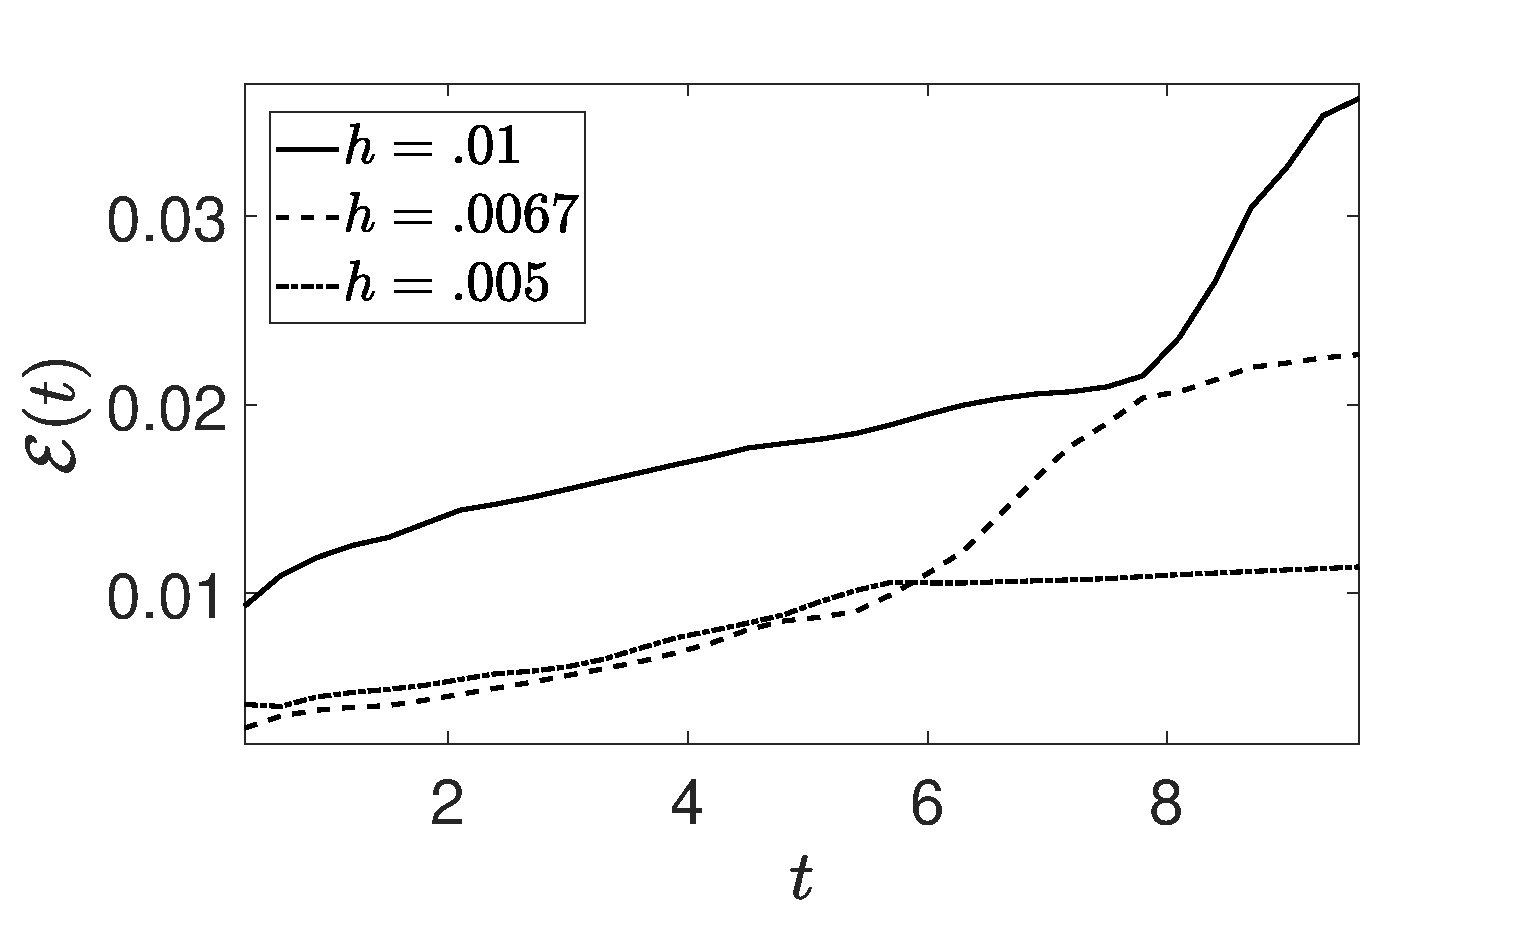
\includegraphics[width=.85\textwidth]{full_error_comparison}\\
(a) $\omega_{m}=1$\\
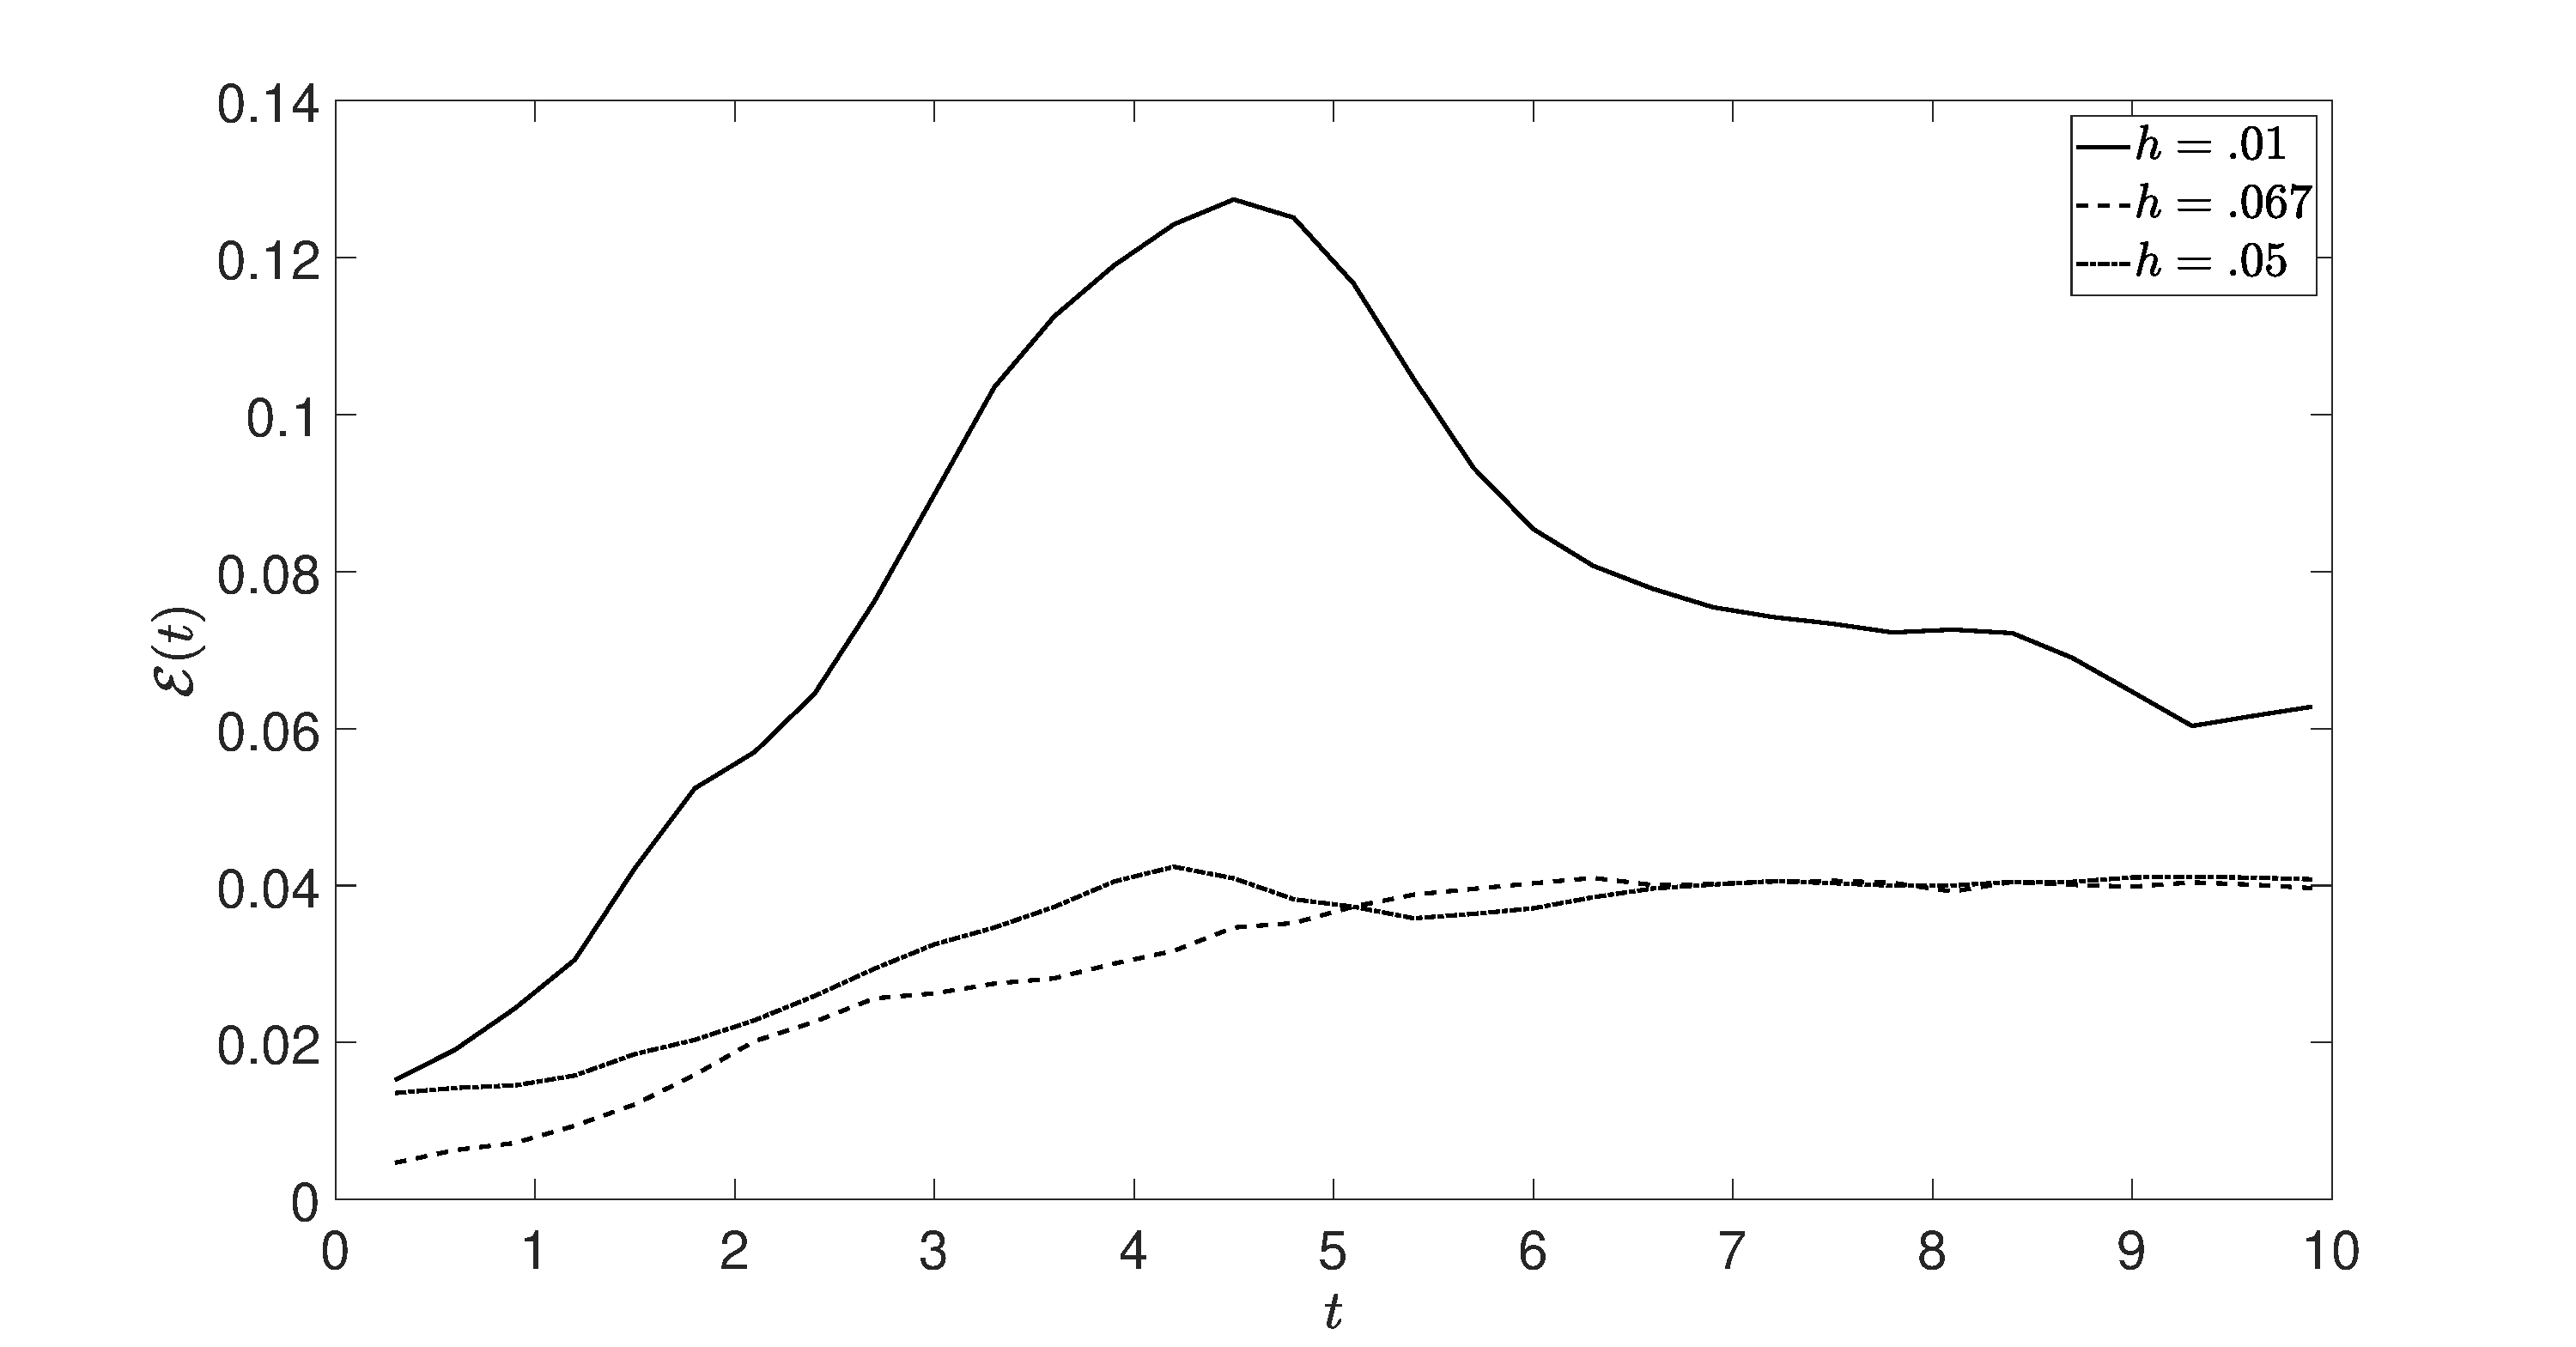
\includegraphics[width=.85\textwidth]{full_error_comparison_wm_10}\\
(b) $\omega_{m}=10$
\end{tabular}
\caption{Error profiles for $h=.005, ~ .0067$, and $.01$ with $\delta=2h$, $\omega_{m}=1$ (a), $\omega_{m}=10$ (b), and regridding done at every six time steps of the simulation.}
\label{fig:err_prof}
\end{figure}

However, the accuracy of the method must be contrasted against the computational expense incurred by introducing greater number of point-vortices at each regridding event.  If we define $N_{s}$ to be the initial number of point vortices and $N_{f}$ to be the final number, we get the following table for differing values of $h$ over the time interval $0\leq t \leq t_{f}$.
\begin{table}
\centering
\begin{tabular}{c|cc}
$h$ & $N_{s}$ & $N_{f}$\\
\hline
.005 & 1252 & 11221\\
.0067 & 698 & 8385\\
.01 & 308 & 5937
\end{tabular}
\caption{For varying grid spacings, $h$, the starting particle count $N_{s}$ and the ending particle count $N_{f}$.  The increase is a consequence of the regridding procedure, which in this case is done every six time steps of the simulation.  }
\end{table}
Likewise, for the range of vorticity strengths we wish to examine, we see by comparing Figures \ref{fig:err_prof} (a) and (b) that choosing $h=.0067$  provides a relatively high-degree of accuracy while keeping the number of point vortices in the simulation at a more manageable level.  We therefore stick with this particle spacing throughout the rest of the paper.  

The increase in particle count and also position relative to the interior of the vorticity profile also raises the question of newly introduced points running into either the solid boundary at $z=0$ or the free surface at $y=\epsilon\eta(x,t)+1$.  We therefore modify the interpolation scheme so that vortices do not propagate past either $z=0$ or $z=.9$.    Thus, while maintaing the accuracy of the PVM, this approach introduces significant overhead in the computation of particle velocities, which again is ameliorated through the use of a FMM.  

%%%%%%%%%%%%%%%%%%%%%%%%%%%%%%%%%%%%%%%%%%%%%%%%%%%%%%%%%%%%%%%%%%%%%%%%%%%%%%%%%%%
%%%%%%%%%%%%%%%%%%%%%%%%%%%%%%%%%%%%%%%%%%%%%%%%%%%%%%%%%%%%%%%%%%%%%%%%%%%%%%%%%%%
\section{Results}
Throughout this section, we take $L = \lambda M$, where $M$ rougly counts the number of characteristic wavelengths included in the computational domain.   Correspondingly, we take $M=\mathcal{K}(\tilde{m})/\kappa$, so that the period of the numerical simulation is equal to the period of the cnoidal wave.   We note that this does place some limits on the overalll elliptic modulus we may pick since as $\tilde{m}\rightarrow 1^{-}$, the solitary wave limit moves the periodic copies of the of the vortices in the lateral direction off to infinity.  This creates a series of source terms in the free boundary equations which decay only quadratically, thereby radically limiting the efficacy of a spectral method for modeling the surface.  This is a fascinating complication beyond the scope of the present paper, but one that will be explored in future research.  

With regards to the details of the simulations, we let $\mu=.2$, $\gamma = \sqrt{\mu}$, which is consistent with the KdV approximation, and $t_{f}=2/\mu$, so that nonlinearity has enough time to have a significant impact.  Twenty terms are taken in the recursive compuation of the DNO, and a total of $K_{T}=512$ modes are used for the pseudospectral approximation of the free surface.  A Runge-Kutta 4 method with integrating factors is used with a time-step of $\delta t = .05$.   We then have for our choice of vortex patch that $F$ is given by 
\[
F = \frac{\pi \omega_{m}R_{v}^{2}}{4\gamma}.
\]
The radius of the patch, $R_{v}$, is chosen so that
\[
R_{v} = \frac{\gamma}{2}\mbox{min}\{1-y_{c},y_{c}\}
\]
where $y_{c}$ is the initial vertical displacement of the patch.  We choose $y_{c}=.35$, so that $R_{v}\approx.1565$.  The initial horizontal displacement is $x_{c}=0$.  The initial position of the wave is at $x=-M/2$.  

With these choices fixed, we note that the unscaled amplitude of the cnoidal wave initial conditions is given by $8(\tilde{m}\kappa)^{2}$.  Throughout our simulations we have chosen $\kappa$ for a given choice of elliptic modulus $\tilde{m}$ so as to make this unscaled amplitude as close to unity as possible while still maintaining convergent numerical simulations.  The issue for convergence in the DNO is a complicated one \cite{guyenne,wilkening}, though the issue then can be mollified by reducing the size of $\mu$.  This of course adds further choices in parameters, which are already numerous as is.  While in this paper we have chosen to stick the with DNO approach due to its relative ease of implementation, there are similar but more stable approaches such as the Transformed Field Expansion \cite{nicholls} which should be adaptable to this problem.  Exploring this issue is a subject of future research.   

In each of the following plots, we look at both the evolution of the vortex patch, and a comparison of the evolution of the free surface from the same initial conditions.  Solid lines correspond to results in which $F\neq0$ while dashed lines correspond to the zero vorticity, or $F=0$, case.  To better understand the impact of vortex patches on the cnoidal wave profiles examined in this work, we also provide a more quantitative measure of the impact of the vortex patch.  This is done by plotting a relative comparison of the total energy in the surface, where the total energy in the surface in the shallow-water coordinates is given by 
\[
E(t;F) = \frac{1}{2}\int_{-M}^{M} \left(q G(\eta)Q  + \eta^{2}\right)dx,
\]
where we have emphasized the role of the patch through the implicit inclusion of the paramter $F$.  In the absence of a vortex patch, i.e. $F=0$, $E(t;0)$ is a conserved quantity of the flow since it serves as the Hamiltonian of the dynamical system describing the surface dynamics \cite{zakharov}.  Thus, in the following figures, we plot the relative difference in energy $\delta E(t;F)$ where
\[
\delta E(t;F) = \frac{E(t;F)-E(t;0)}{E(t;0)}.
\]
%%%%%%%%%%%%%%%%%%%%%%%%%%%%%%%%%%%%%%%%%%%%%%%%%%%%%%%%%%%%%%%%%%%%%%%%%%%%%%%%%%%
\subsection*{Elliptic Modulus $\tilde{m}=.3$}
Taking $\tilde{m}=.3$ and $\kappa = .5$, this corresponds to $M \approx 3.3$.  Taking $K_{T}=512$, this gives $\delta x = .013$.  The unscaled amplitude of the cnoidal initial conditions is given by $8(\tilde{m}\kappa)^{2}\approx .18$.  From both the pointwise comparisons in Figure \ref{fig:lowsolwave} and the relative energy inputs in Figure \ref{fig:lowsolenergy}, we see that stronger vorticity corresponds to greater deformation of the surface wave relative to the undisturbed case, and comparing across Figures \ref{fig:midsolwave} and \ref{fig:highsolwave}, we see that the vortex patch has the strongest impact on the least nonlinear waves.  
\begin{figure}
\centering
\begin{tabular}{cc}
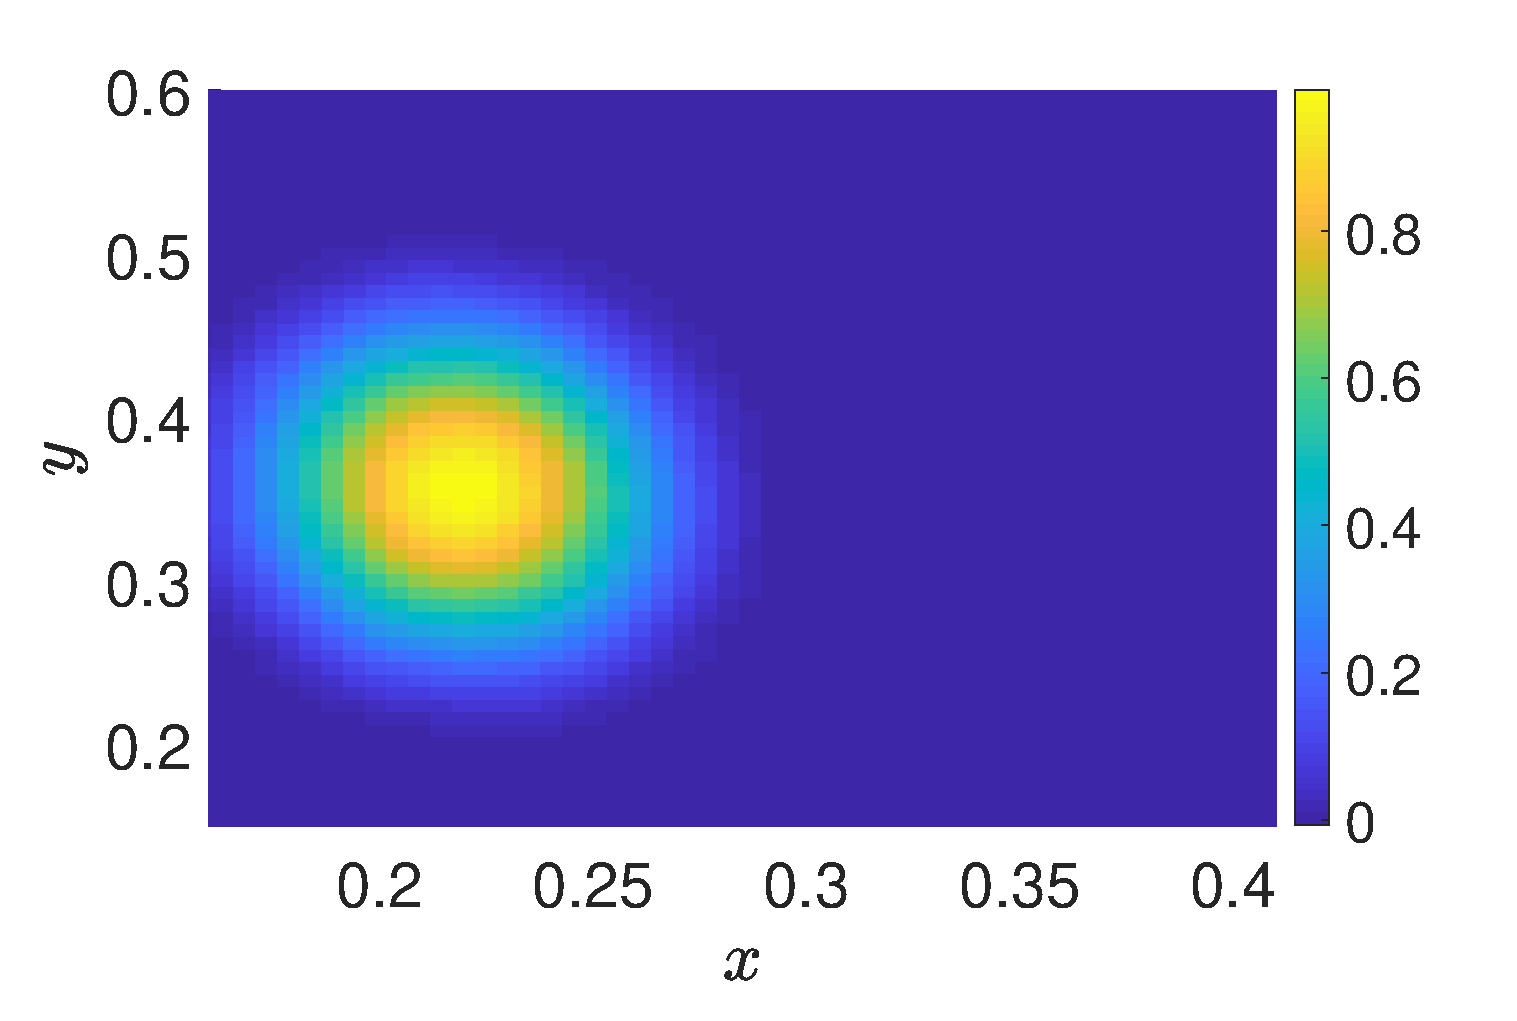
\includegraphics[width=.45\textwidth]{vorticity_wm_1_modu_pt3} & 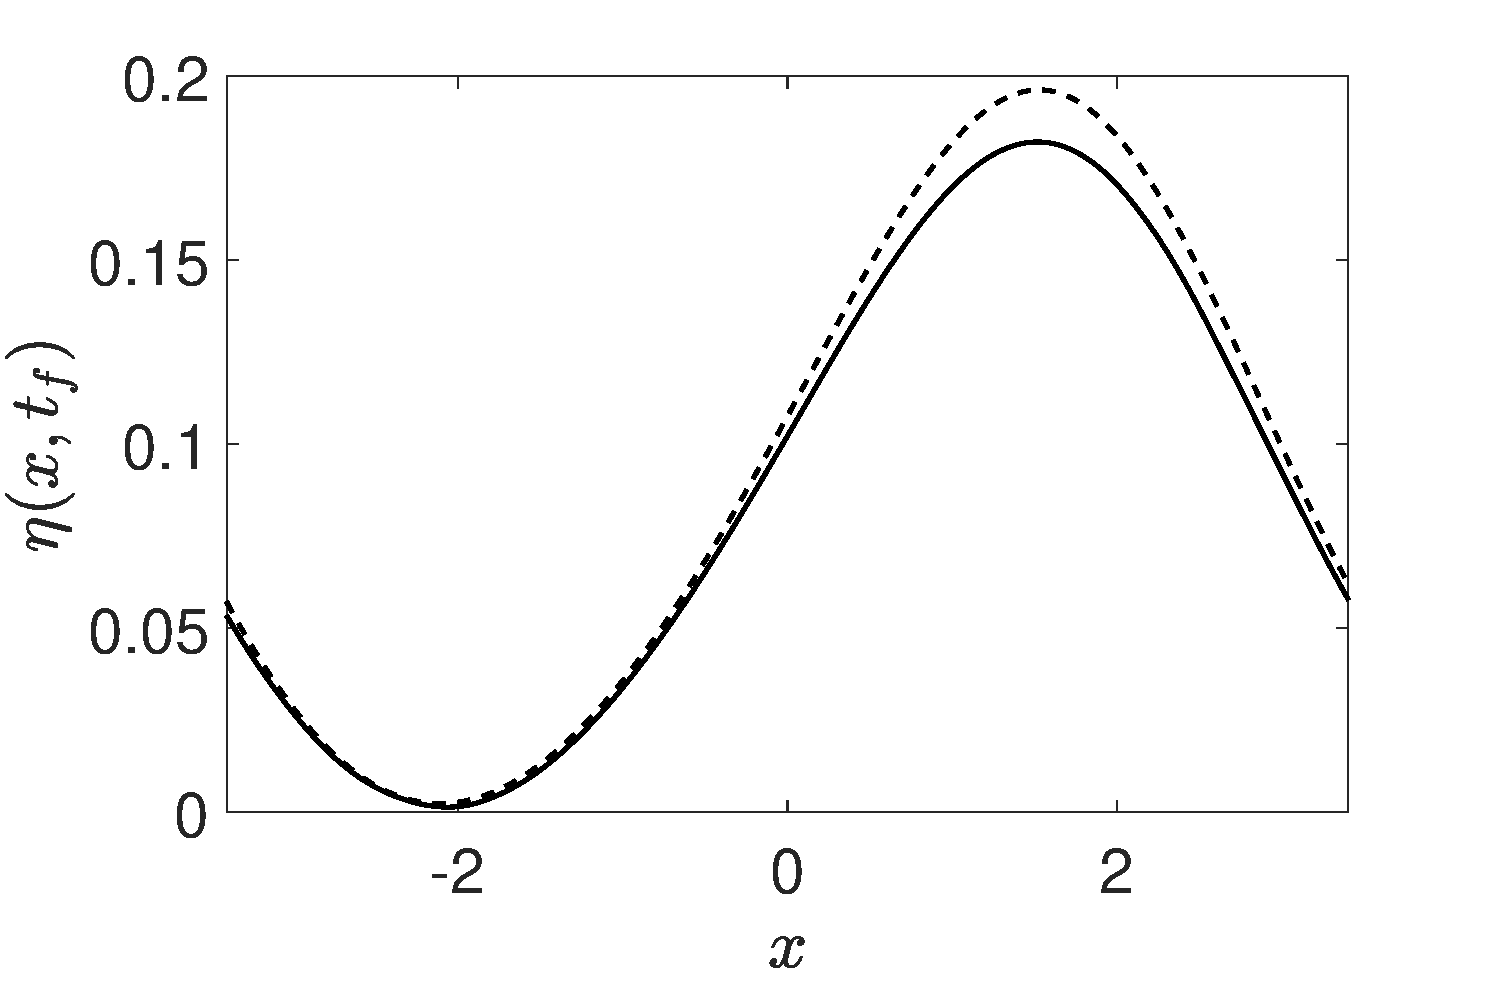
\includegraphics[width=.45\textwidth]{profiles_wm_1_modu_pt3}\\
(a)  $F=.01$ & (b)  $F=.01$\\
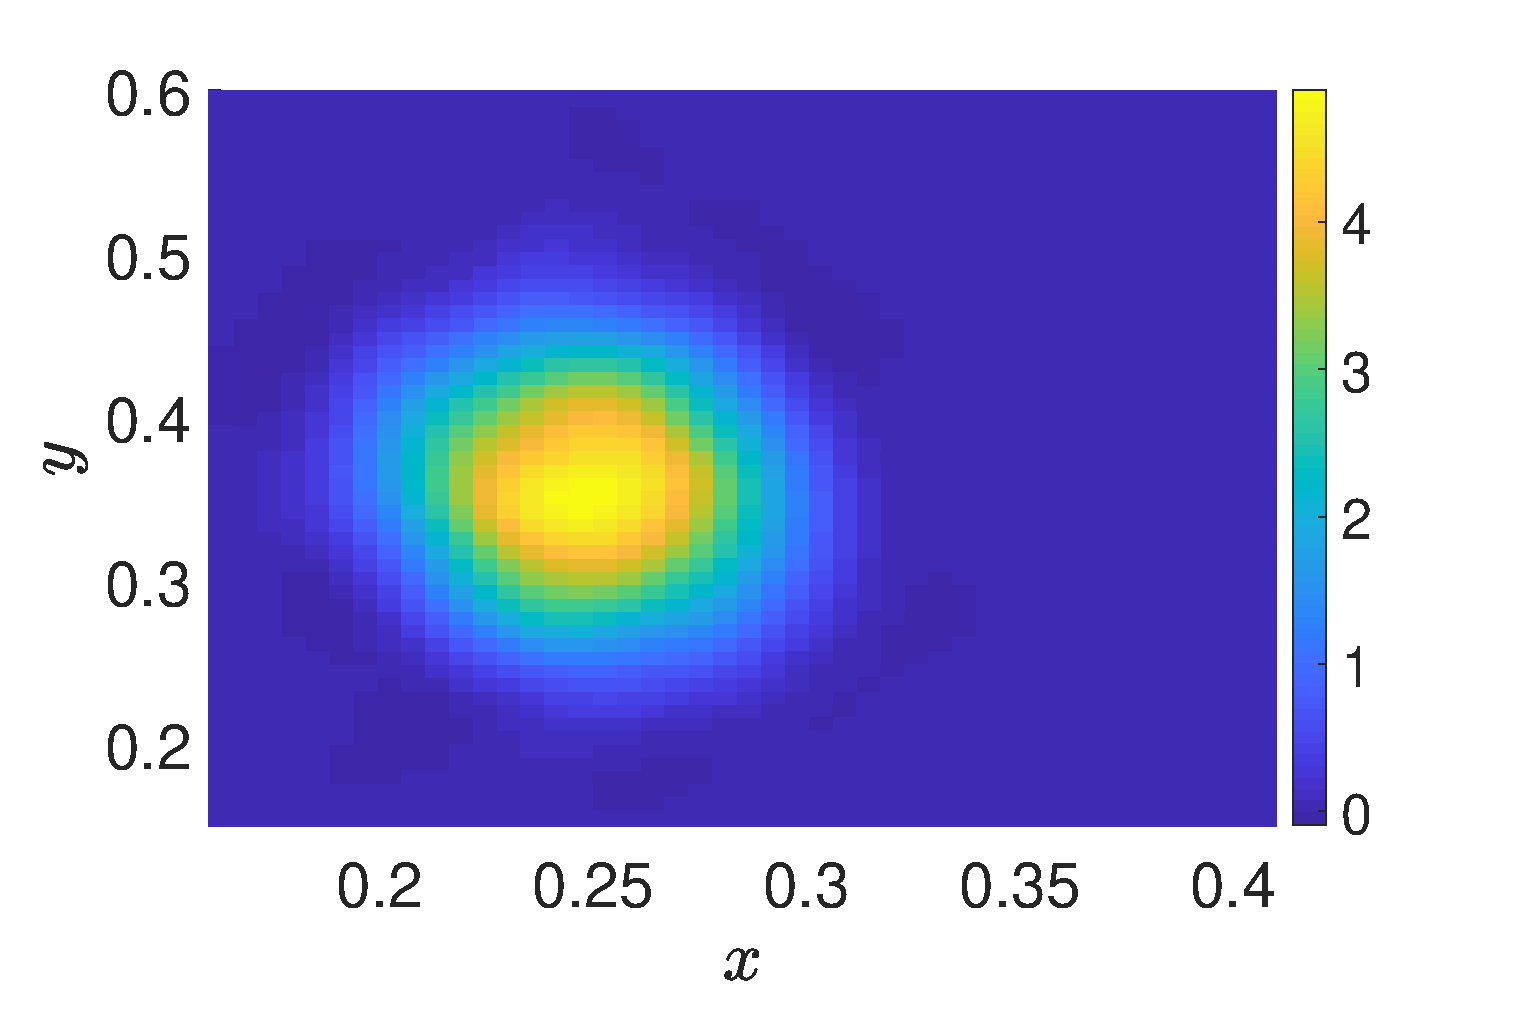
\includegraphics[width=.45\textwidth]{vorticity_wm_5_modu_pt3} & 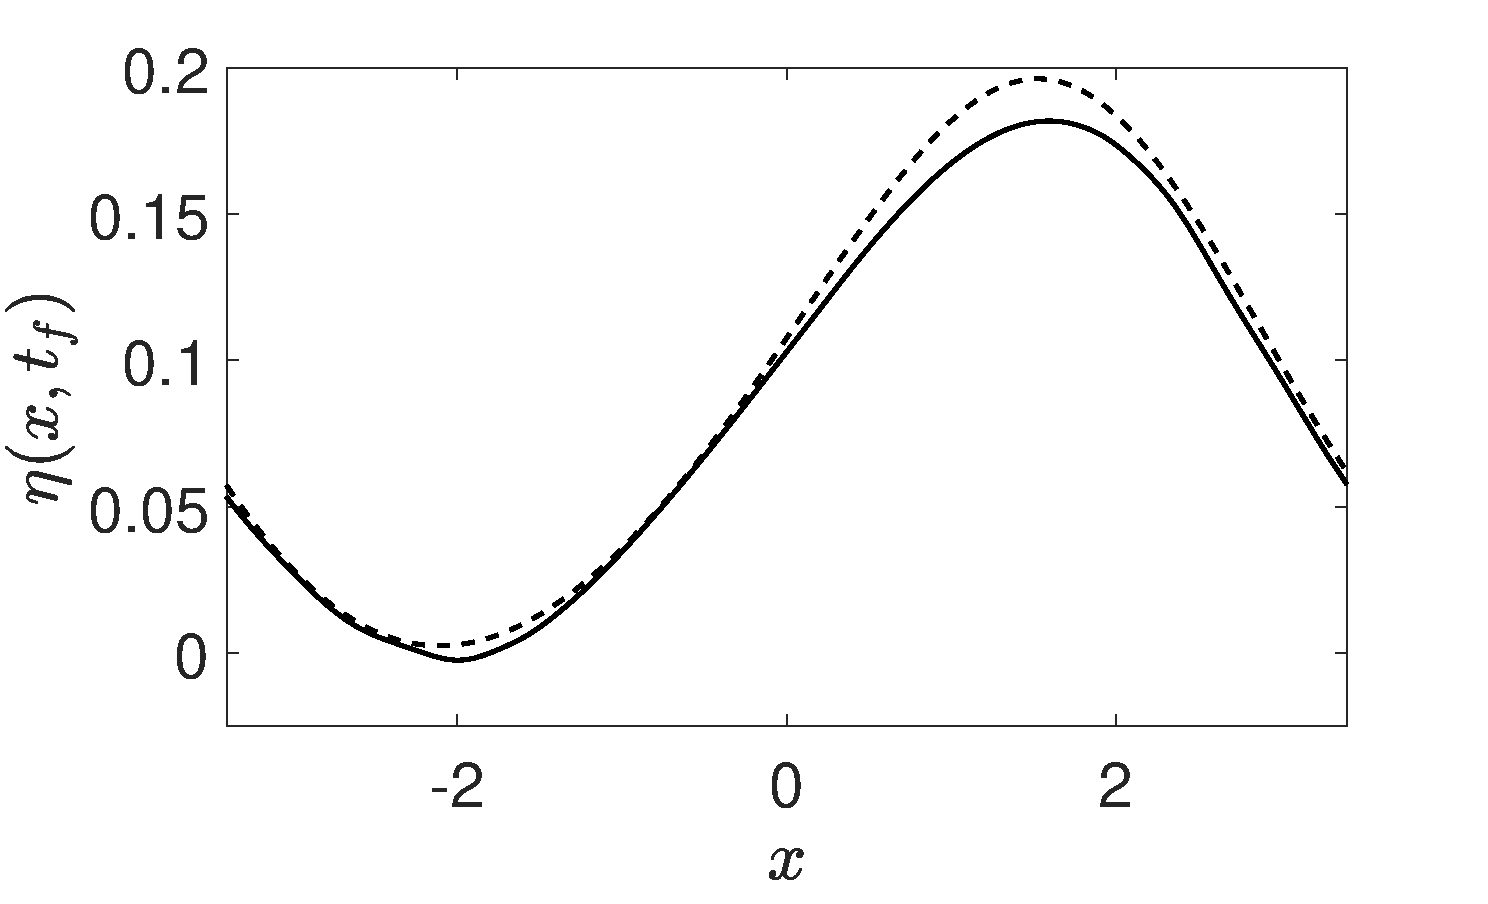
\includegraphics[width=.45\textwidth]{profiles_wm_5_modu_pt3}\\
(c)  $F=.05$ & (d)  $F=.05$\\
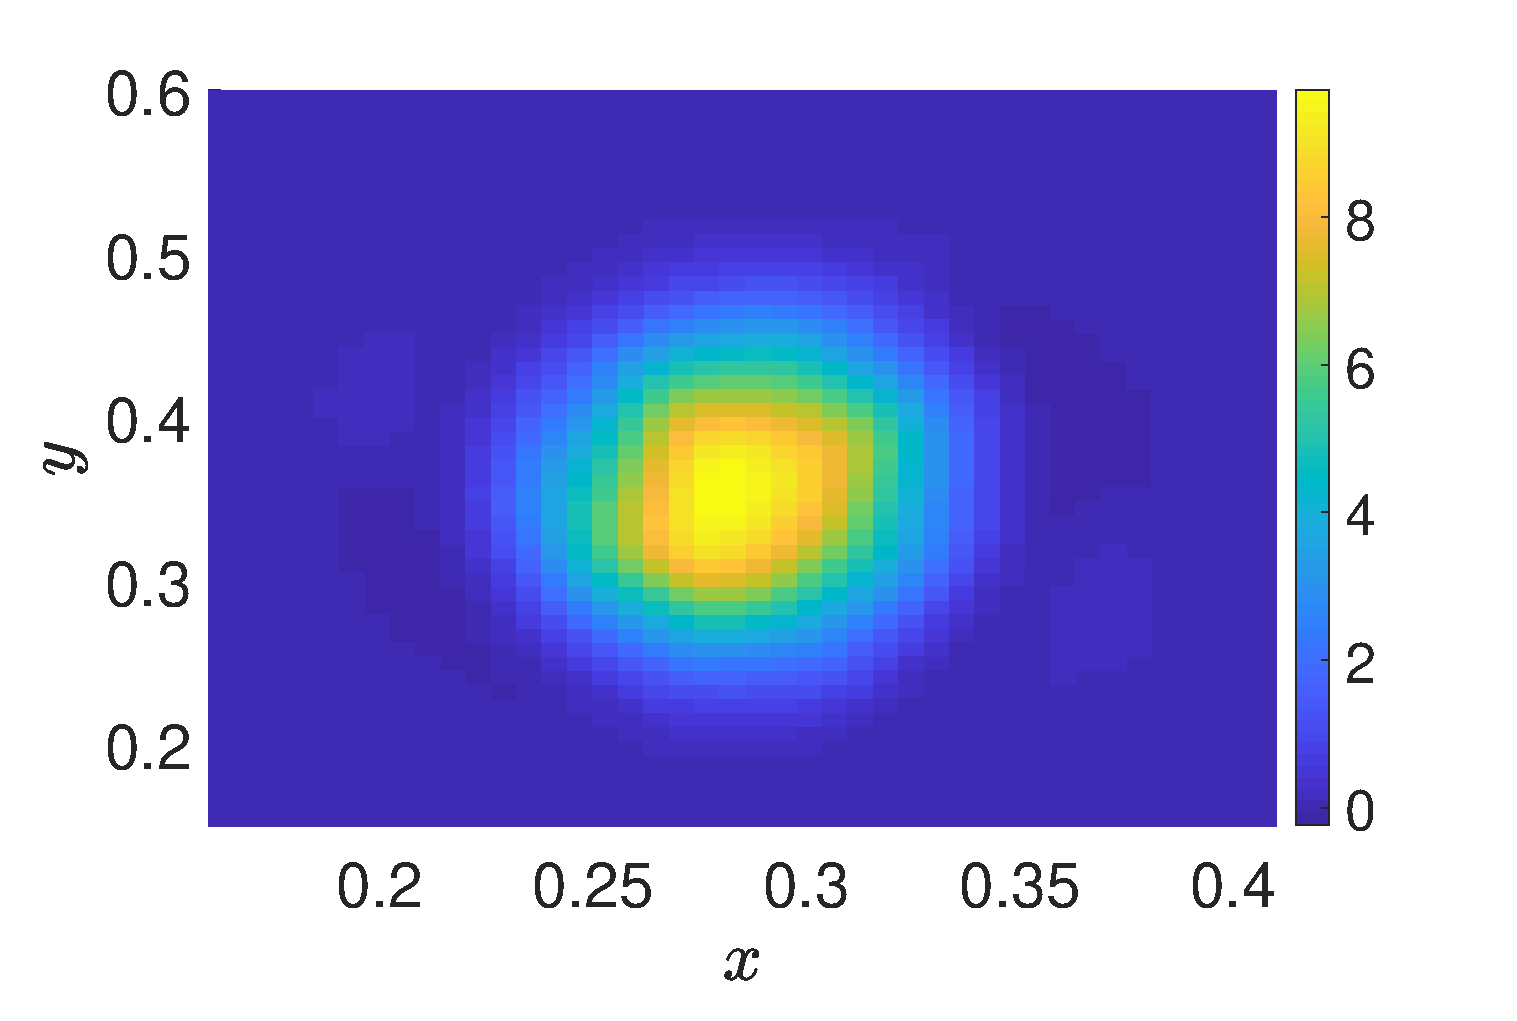
\includegraphics[width=.45\textwidth]{vorticity_wm_10_modu_pt3} & 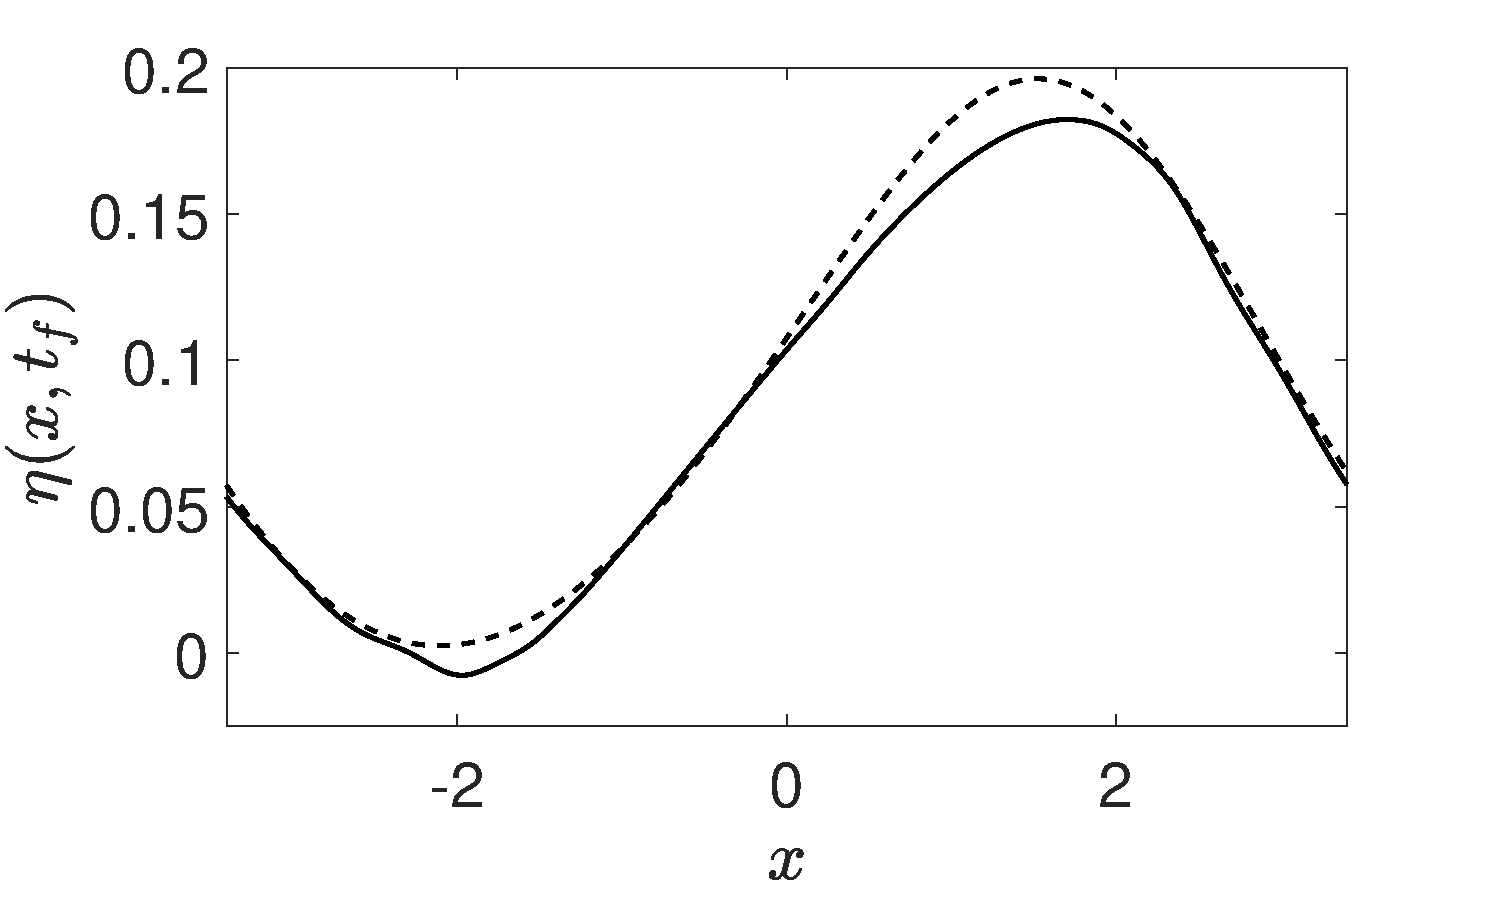
\includegraphics[width=.45\textwidth]{profiles_wm_10_modu_pt3}\\
(e)  $F=.1$ & (f)  $F=.1$
\end{tabular}
\caption{The vortex patches are shown on the left for various values of Froude number $F$, while comparisons of a cnoidal wave over a vortex patch(-) to a cnoidal wave over an irrotational fluid (--) are shown on the right.  Relative to the initial horizontal displacement of $x_{c}=0$, the center of the patch is now between $.2$ and $.3$.  Here $\mu=.2$, $\gamma=\sqrt{\mu}$, $t_{f}=2/\mu$, $\tilde{m}=.3$, $\kappa = .5$.}
\label{fig:lowsolwave}
\end{figure}

\begin{figure}
\centering
\begin{tabular}{cc}
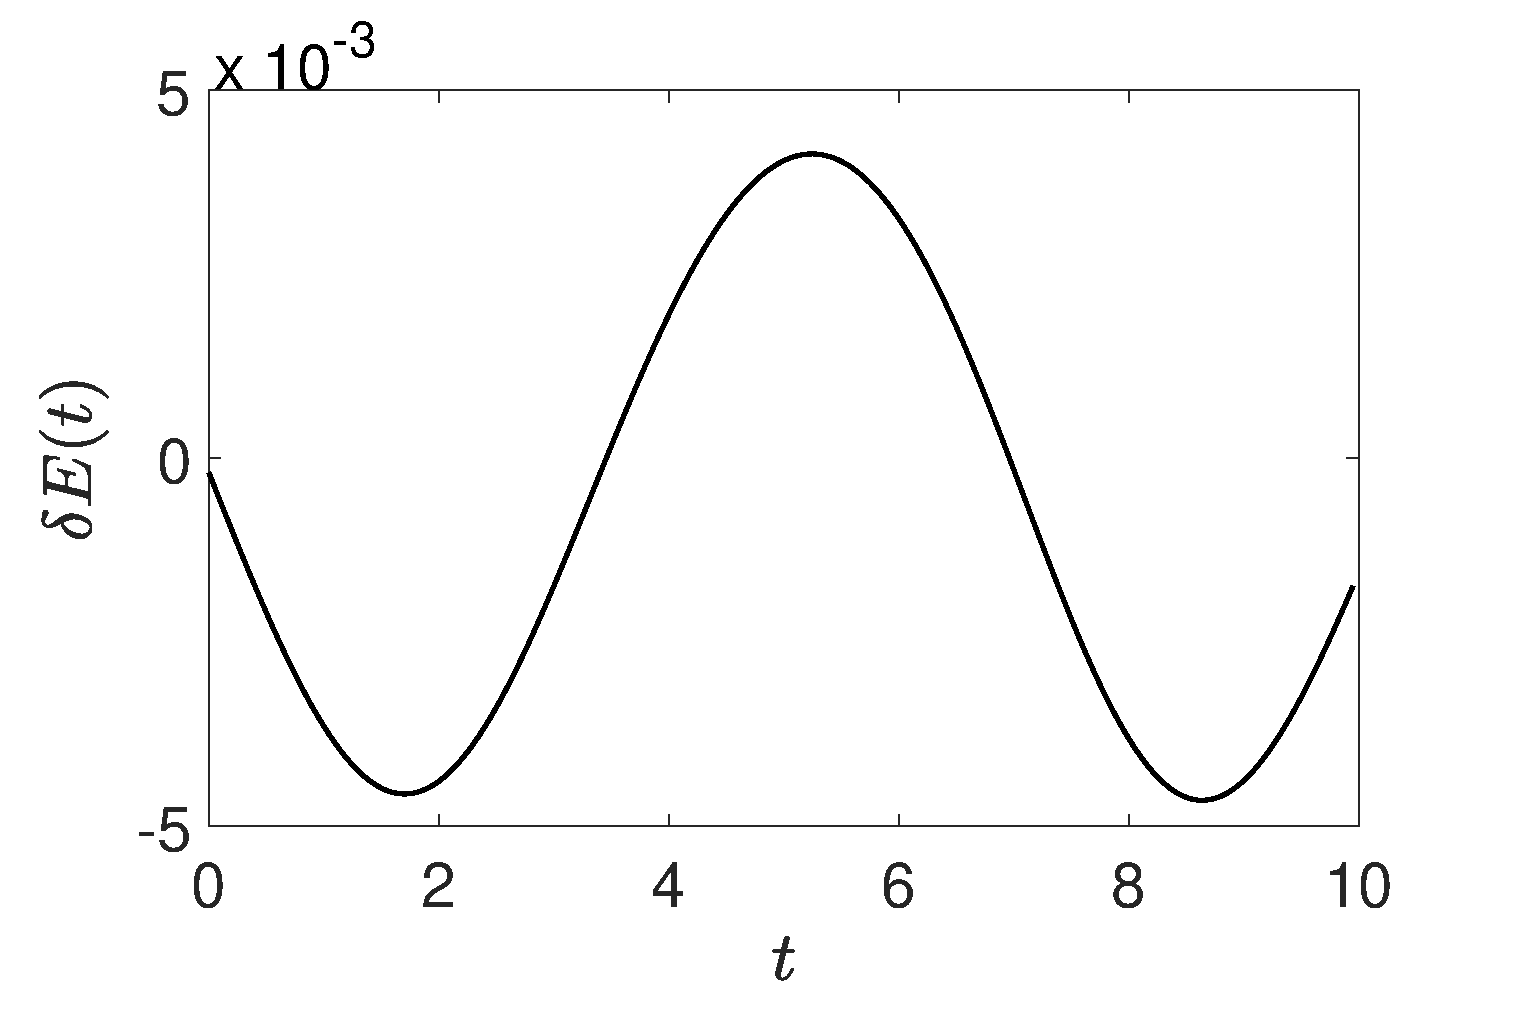
\includegraphics[width=8cm,height=6cm]{energy_wm_1_modu_pt3} & 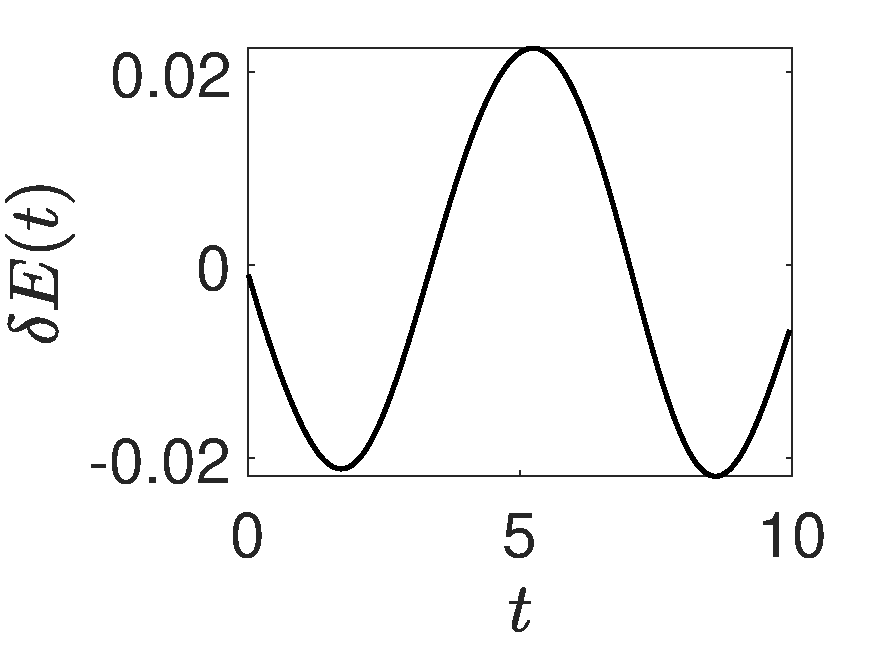
\includegraphics[width=8cm,height=6cm]{energy_wm_5_modu_pt3} \\
(a) $F=.01$ & (b) $F=.05$\\
 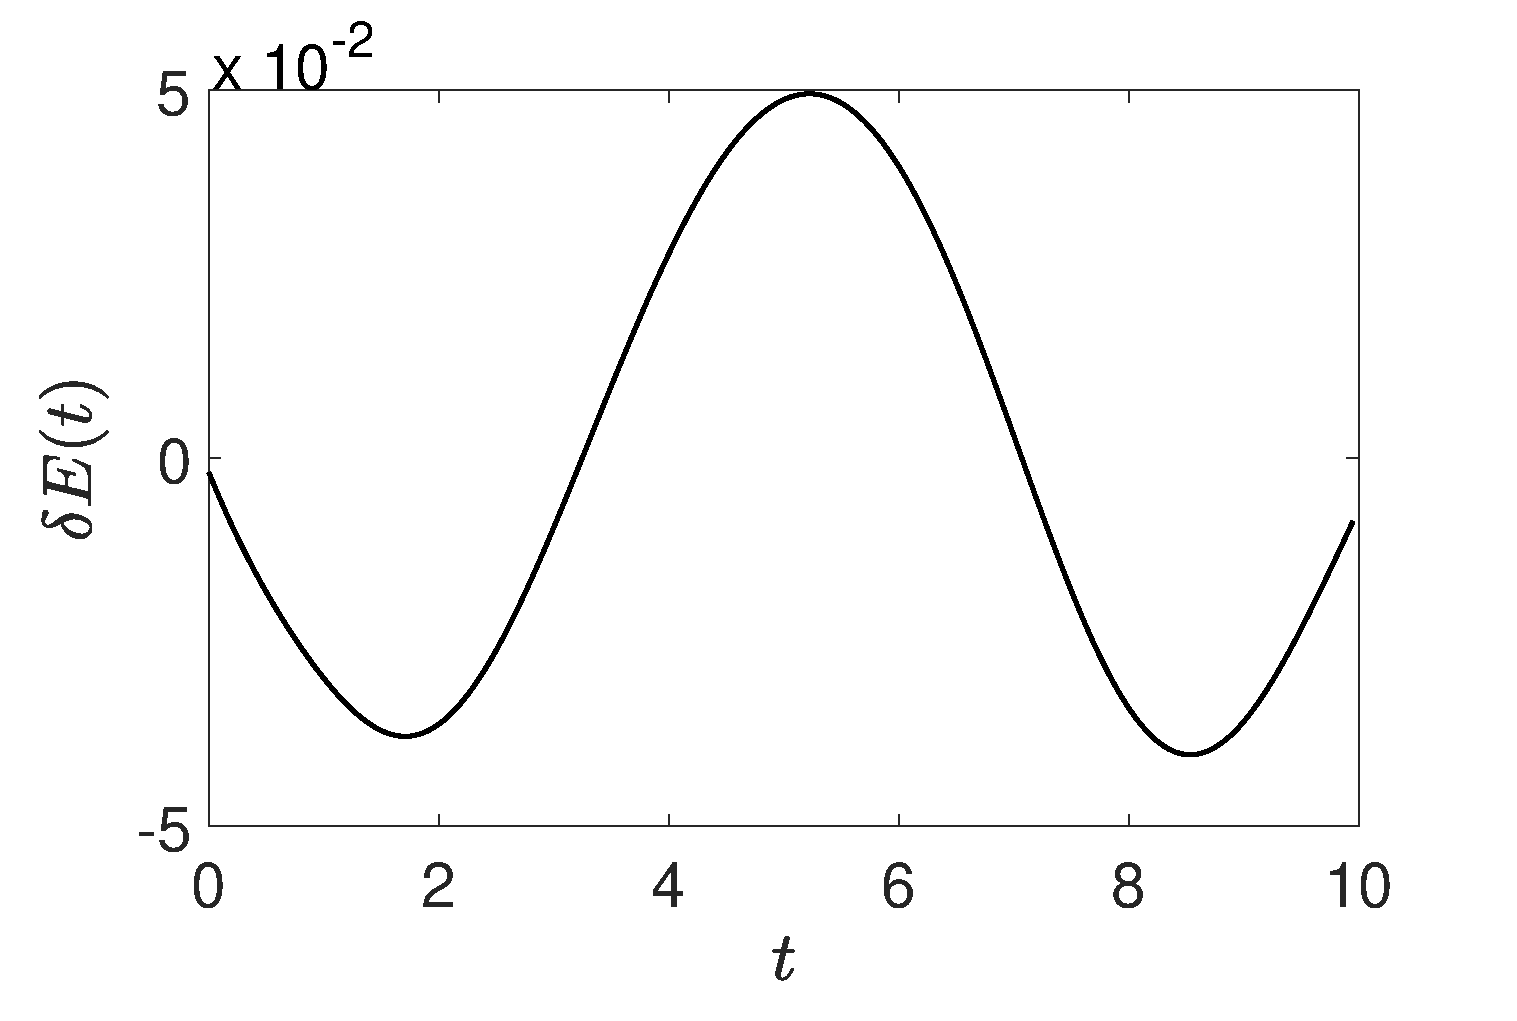
\includegraphics[width=8cm,height=6cm]{energy_wm_10_modu_pt3}\\
 (c) $F=.1$
\end{tabular}
\caption{The relative energy change $\delta E(t)$ for $F=.01$ (a), $F=.05$ (b), and $F=.1$ (c) for $\tilde{m}=.3$ and $\kappa = .5$.  In the relatively weak nonlinearity case, the increasing Froude number leads to greater asymmetry between the maximum and minimum values of the relative energy change, so that the relatively weak nonlinear wave clearly absorbs more energy than it loses when $F=.1$.}
\label{fig:lowsolenergy}
\end{figure}

Moreover, we see that the response of the relative energy input $\delta E(t;F)$ is nonlinear in $F$, with positive peaks being significantly enhanced over negative troughs.  This explains the strong deformations seen in comparing Figures \ref{fig:lowsolwave} (a), (b), and (c) and shows how for a relatively linear surface profile, the vortex patch becomes a source of nonlinear interaction and wave mixing.    We also see that the center of the patch is only moderately displaced relative to its starting position, even accounting for the impact of the image vortices due to the solid boundary at $z=0$.  Were the solid boundary to have that much more of an effect, we should see a greater relative displacment across a ten-fold increase in $F$, which is not present by observing the left-hand side of Figure \ref{fig:lowsolwave}.
%%%%%%%%%%%%%%%%%%%%%%%%%%%%%%%%%%%%%%%%%%%%%%%%%%%%%%%%%%%%%%%%%%%%%%%%%%%%%%%%%%%
\subsection*{Elliptic Modulus $\tilde{m}=.6$}
Taking $\tilde{m}=.6$, we find that $\kappa = .43$, this corresponds to $M \approx 4.4$.  Taking $K_{T}=512$, this gives $\delta x = .0172$.  The unscaled amplitude of the cnoidal initial conditions is given by $8(\tilde{m}\kappa)^{2}\approx .53$.  As seen in Figure \ref{fig:midsolwave}, we see that the larger elliptic modulus and larger amplitude makes the surface wave less responsive to the impact of vorticity.  Nevertheless, the patch consistently lowers maximum amplitudes, and when large enough, induces significant oscillations in the surface profile.  
\begin{figure}
\centering
\begin{tabular}{cc}
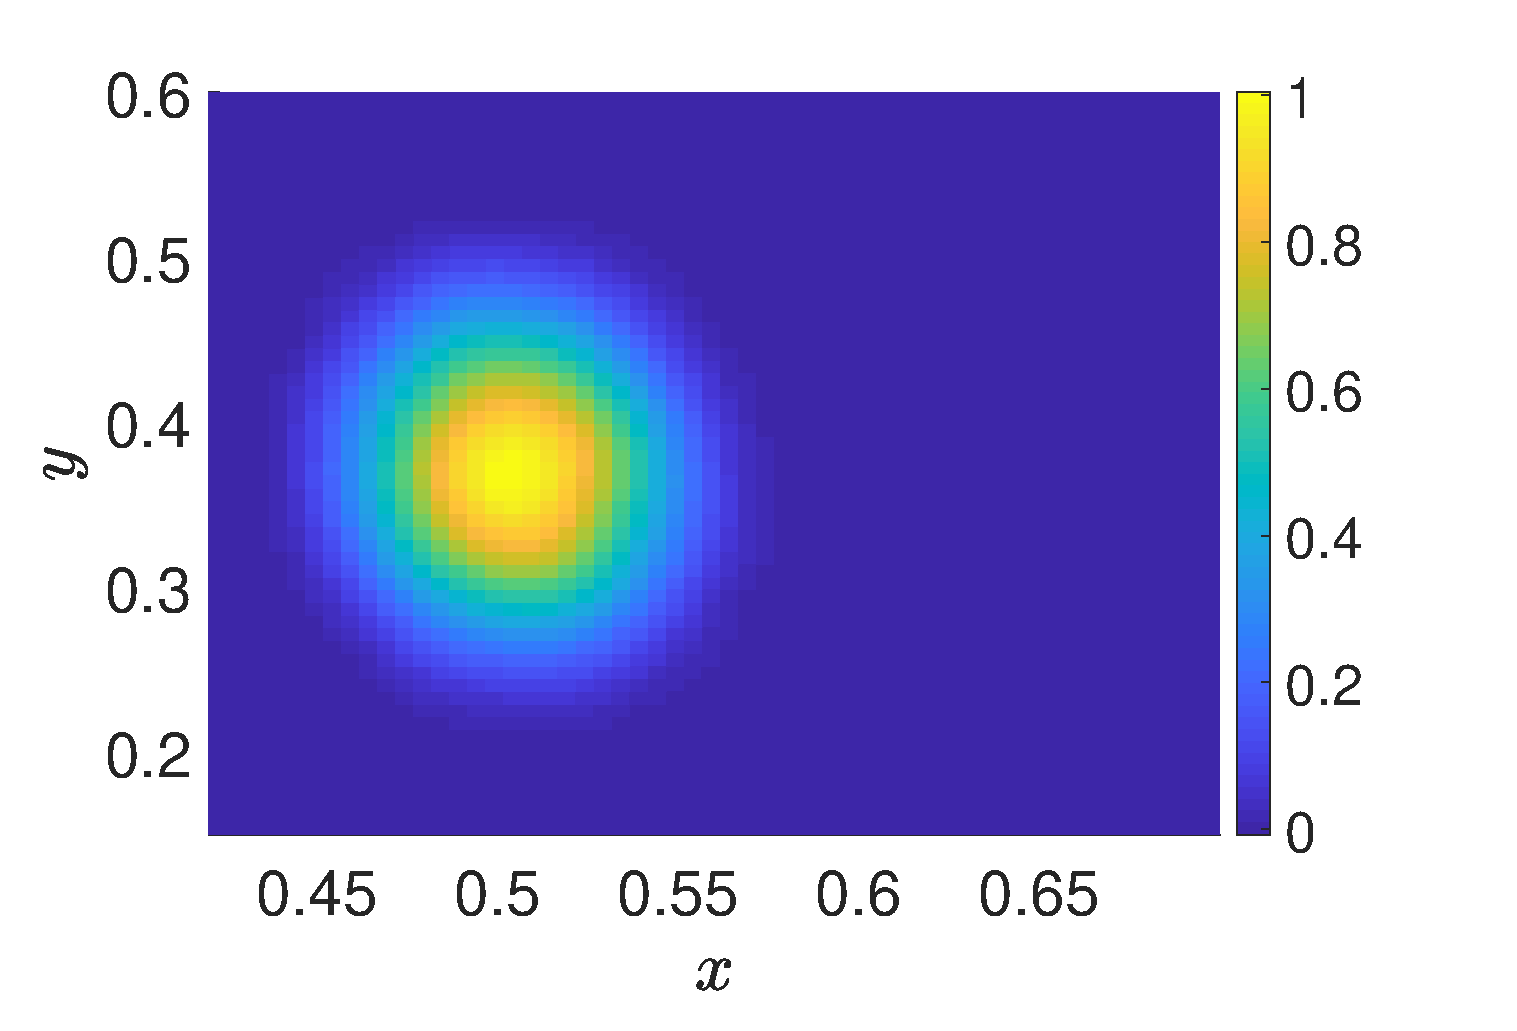
\includegraphics[width=.45\textwidth]{vorticity_wm_1_modu_pt6} & 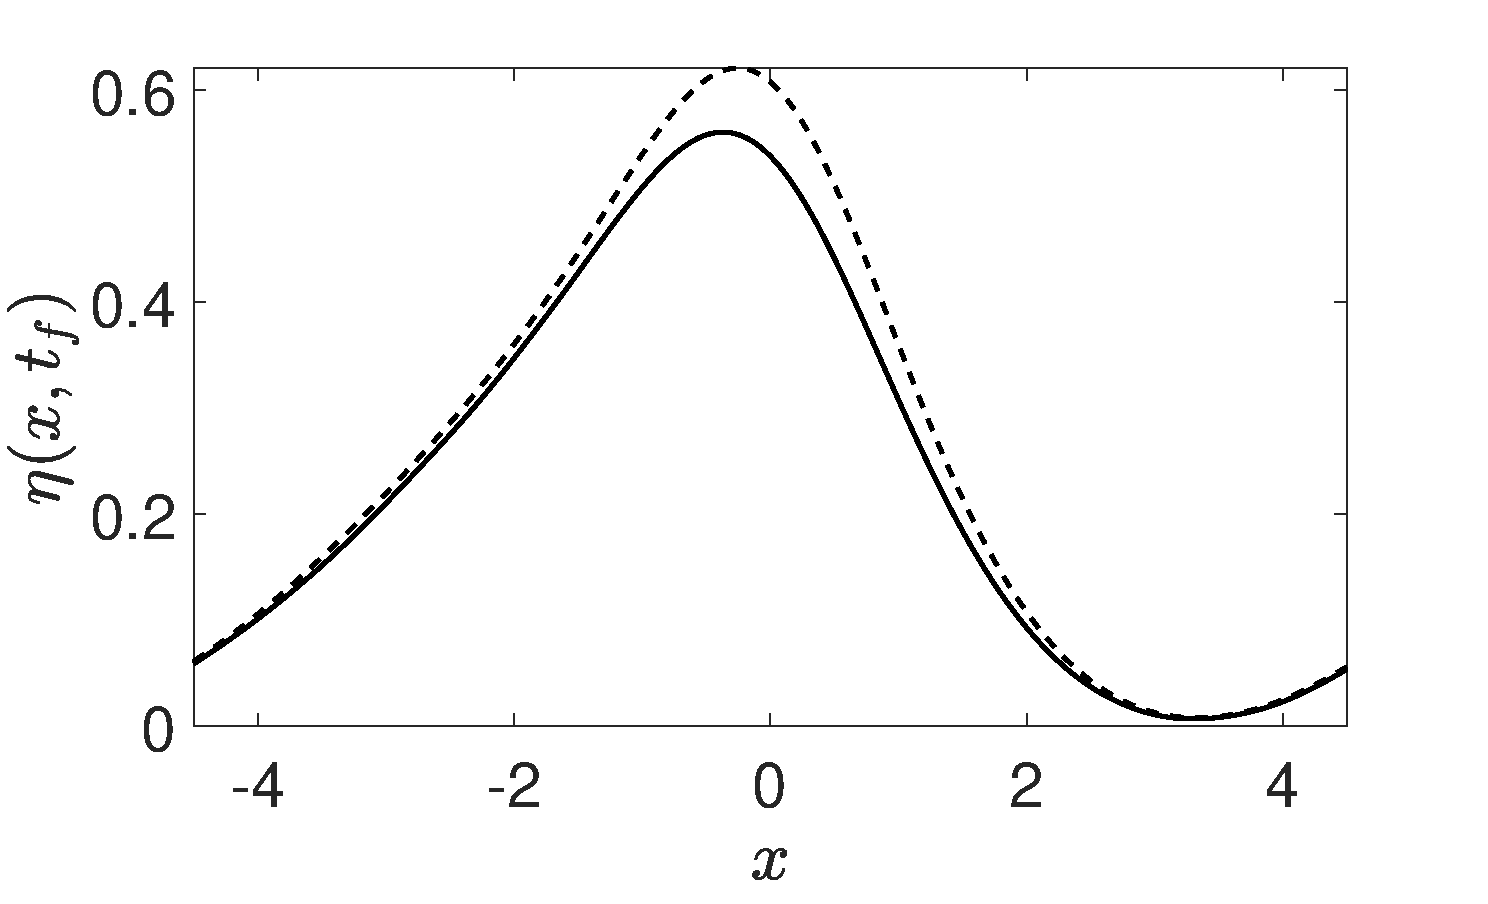
\includegraphics[width=.45\textwidth]{profiles_wm_1_modu_pt6}\\
(a)  $F=.01$ & (b)  $F=.01$\\
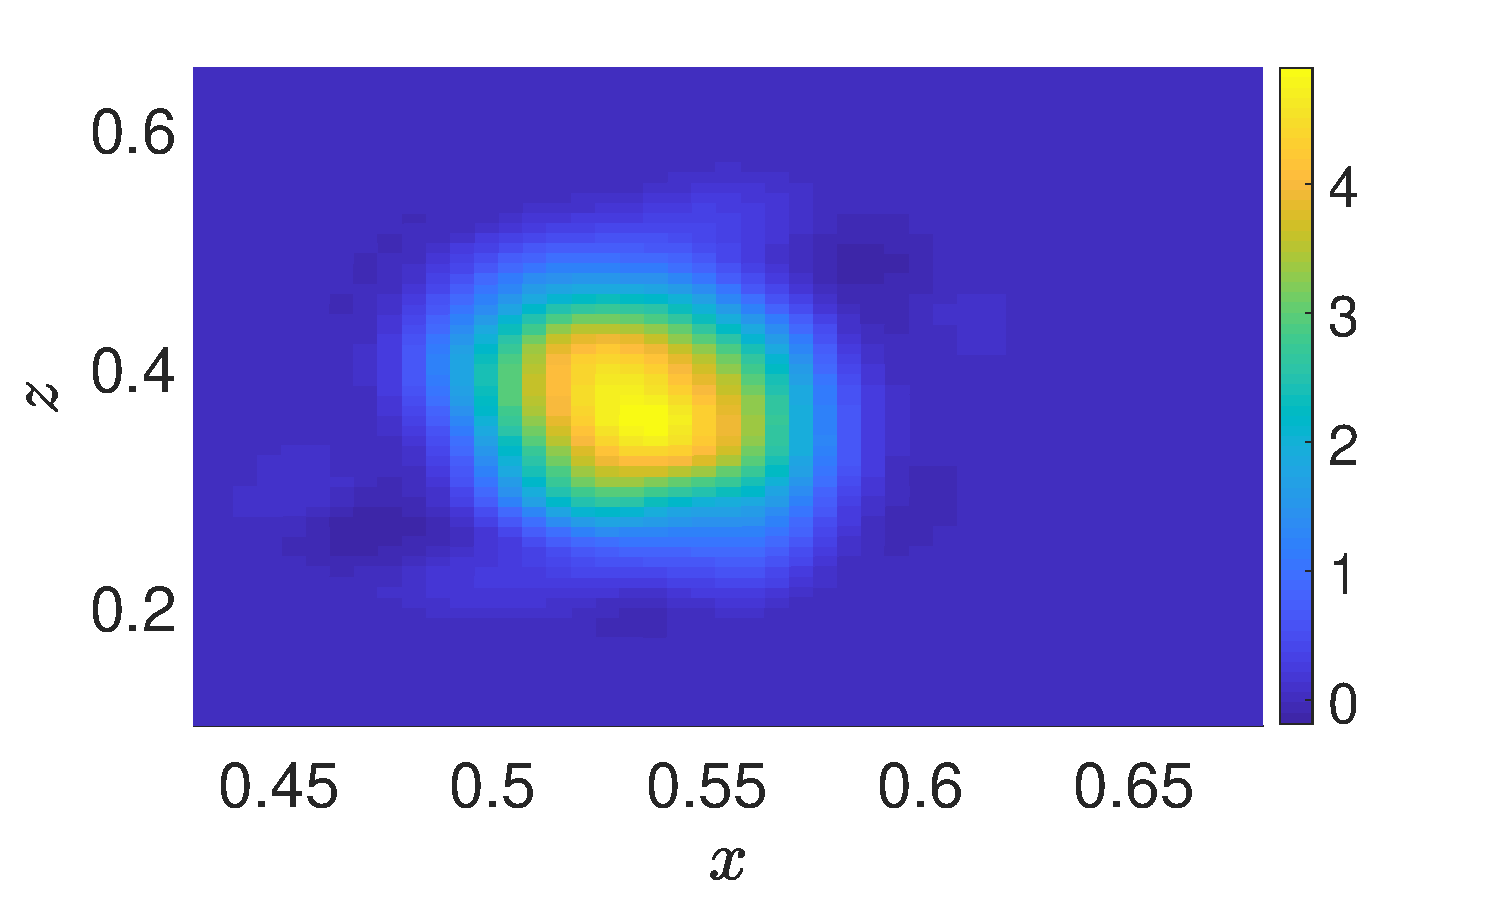
\includegraphics[width=.45\textwidth]{vorticity_wm_5_modu_pt6} & 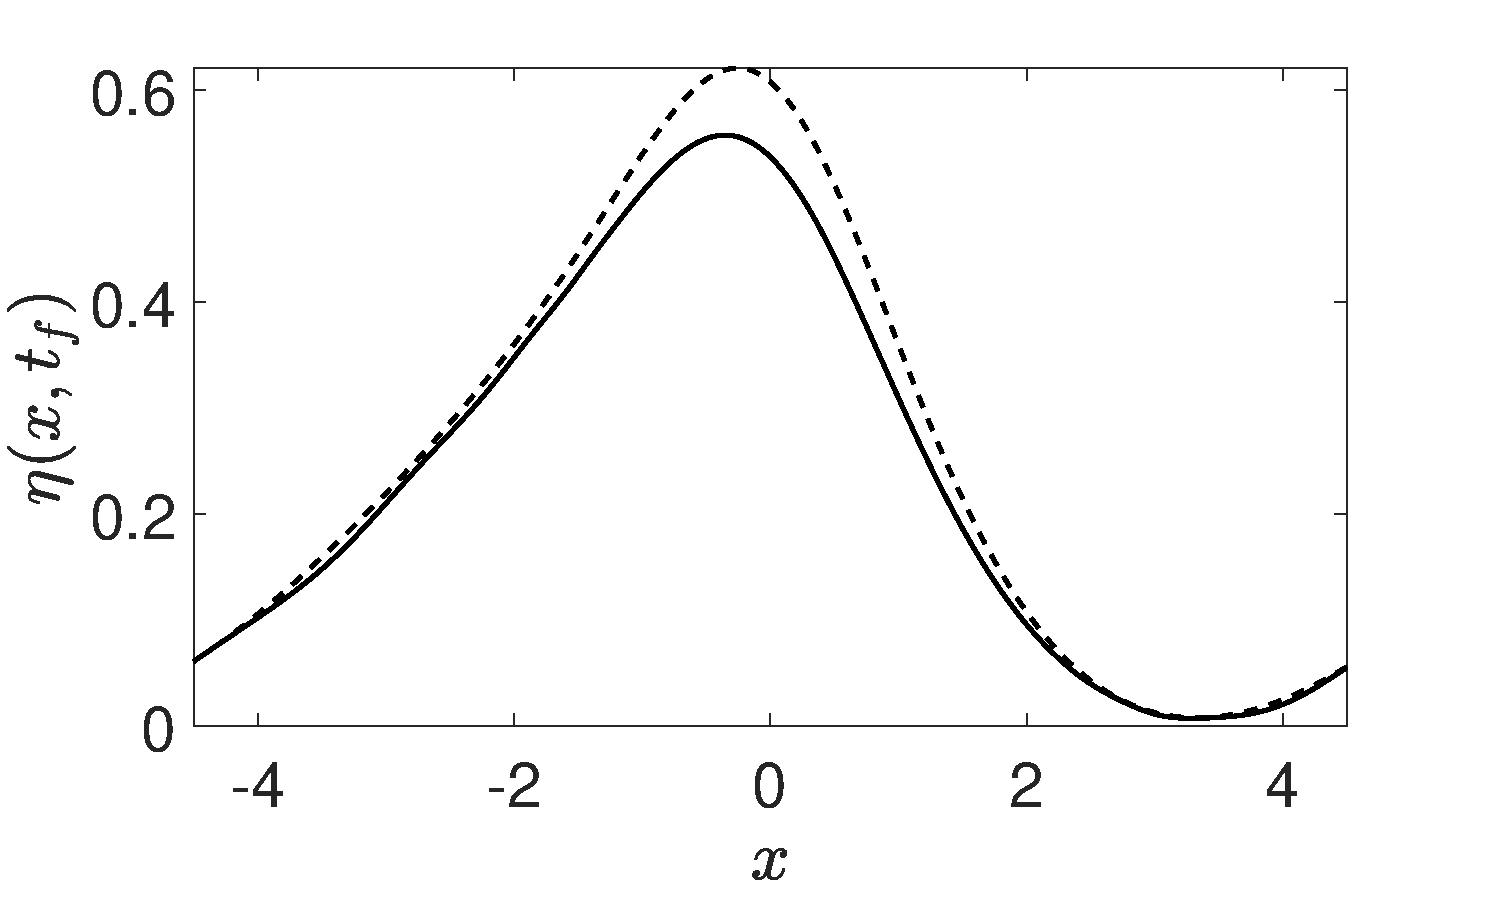
\includegraphics[width=.45\textwidth]{profiles_wm_5_modu_pt6}\\
(c)  $F=.05$ & (d)  $F=.05$\\
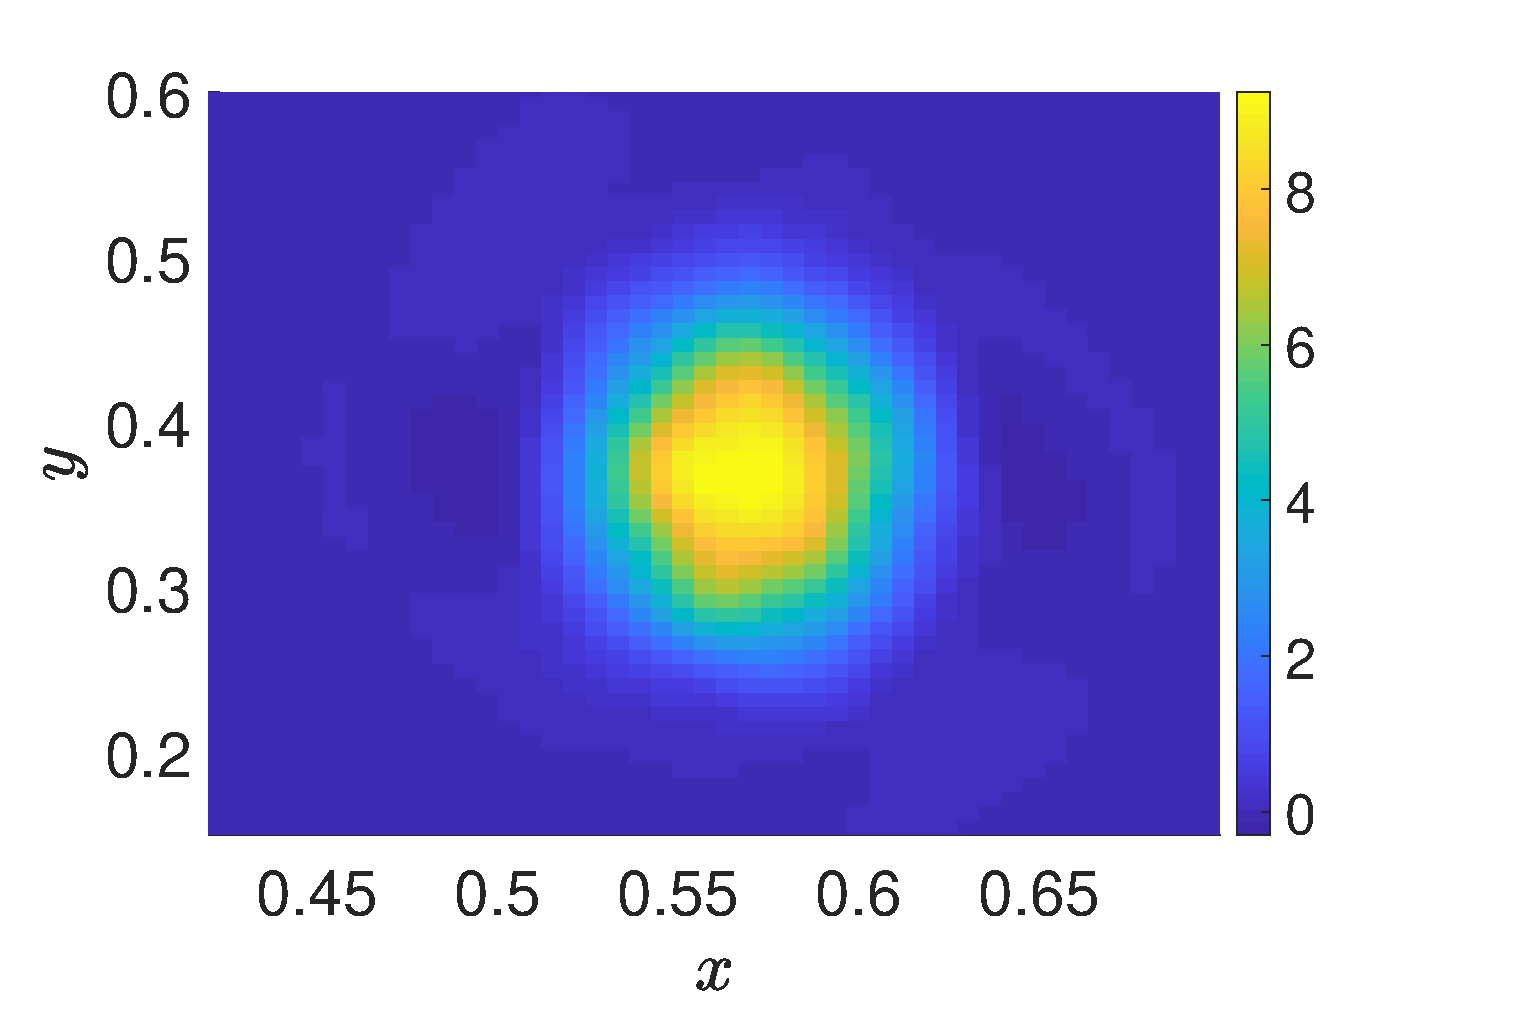
\includegraphics[width=.45\textwidth]{vorticity_wm_10_modu_pt6} & 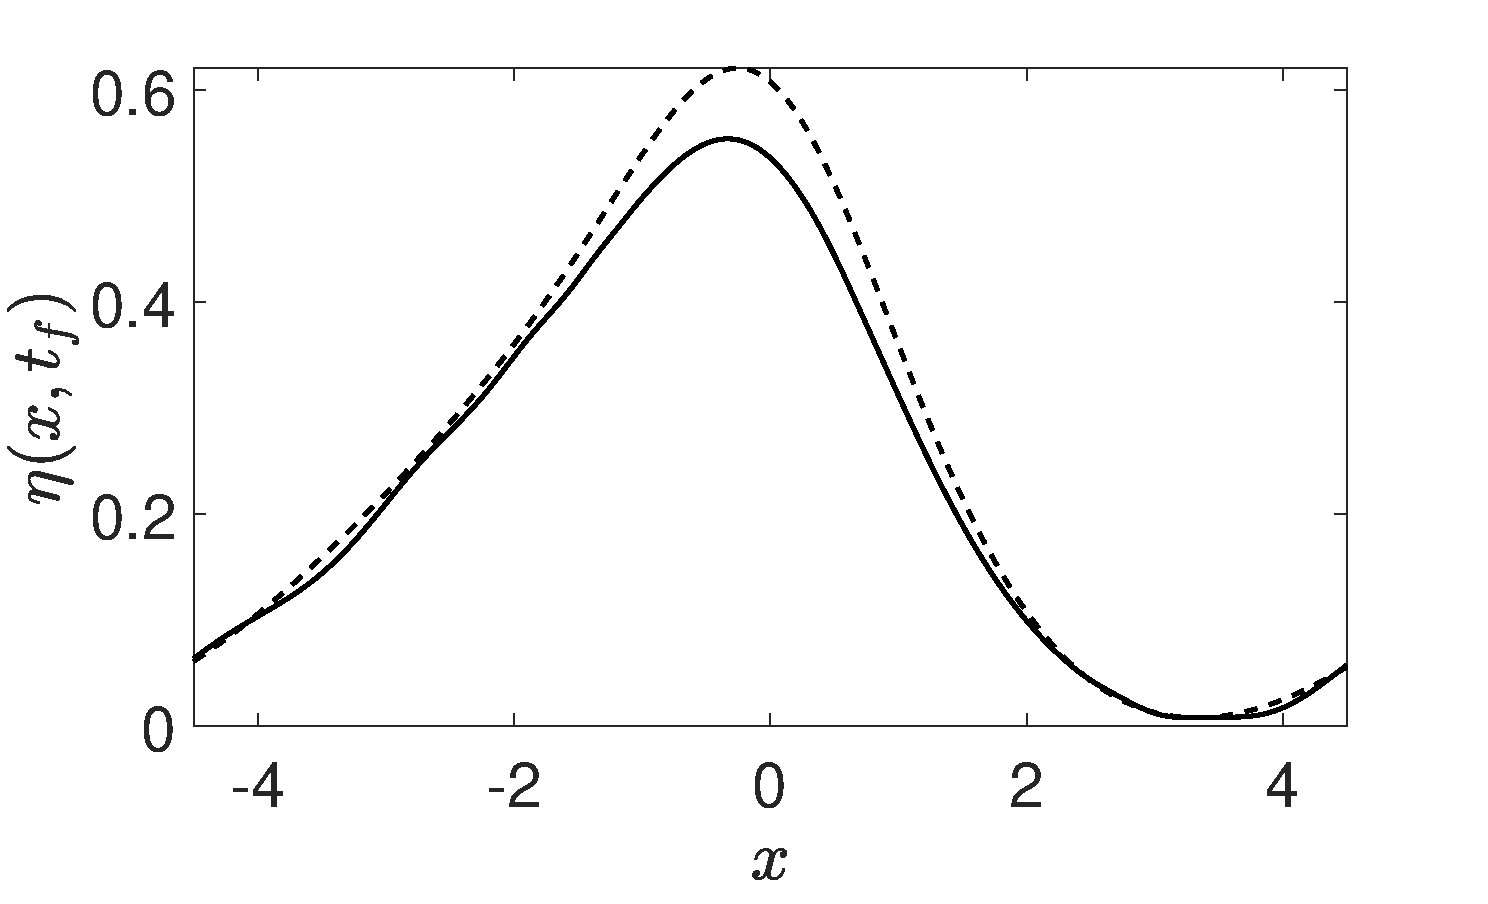
\includegraphics[width=.45\textwidth]{profiles_wm_10_modu_pt6}\\
(e)  $F=.1$ & (f)  $F=.1$
\end{tabular}
\caption{The vortex patches are shown on the left for various values of Froude number $F$, while comparisons of a cnoidal wave over a vortex patch(-) to a cnoidal wave over an irrotational fluid (--) are shown on the right.  Relative to the initial horizontal displacement of $x_{c}=0$, the center of the patch is now between $.5$ and $.6$.  Here $\mu=.2$, $\gamma=\sqrt{\mu}$, $t_{f}=2/\mu$, $\tilde{m}=.6$, $\kappa = .43$.}
\label{fig:midsolwave}
\end{figure}

\begin{figure}
\centering
\begin{tabular}{cc}
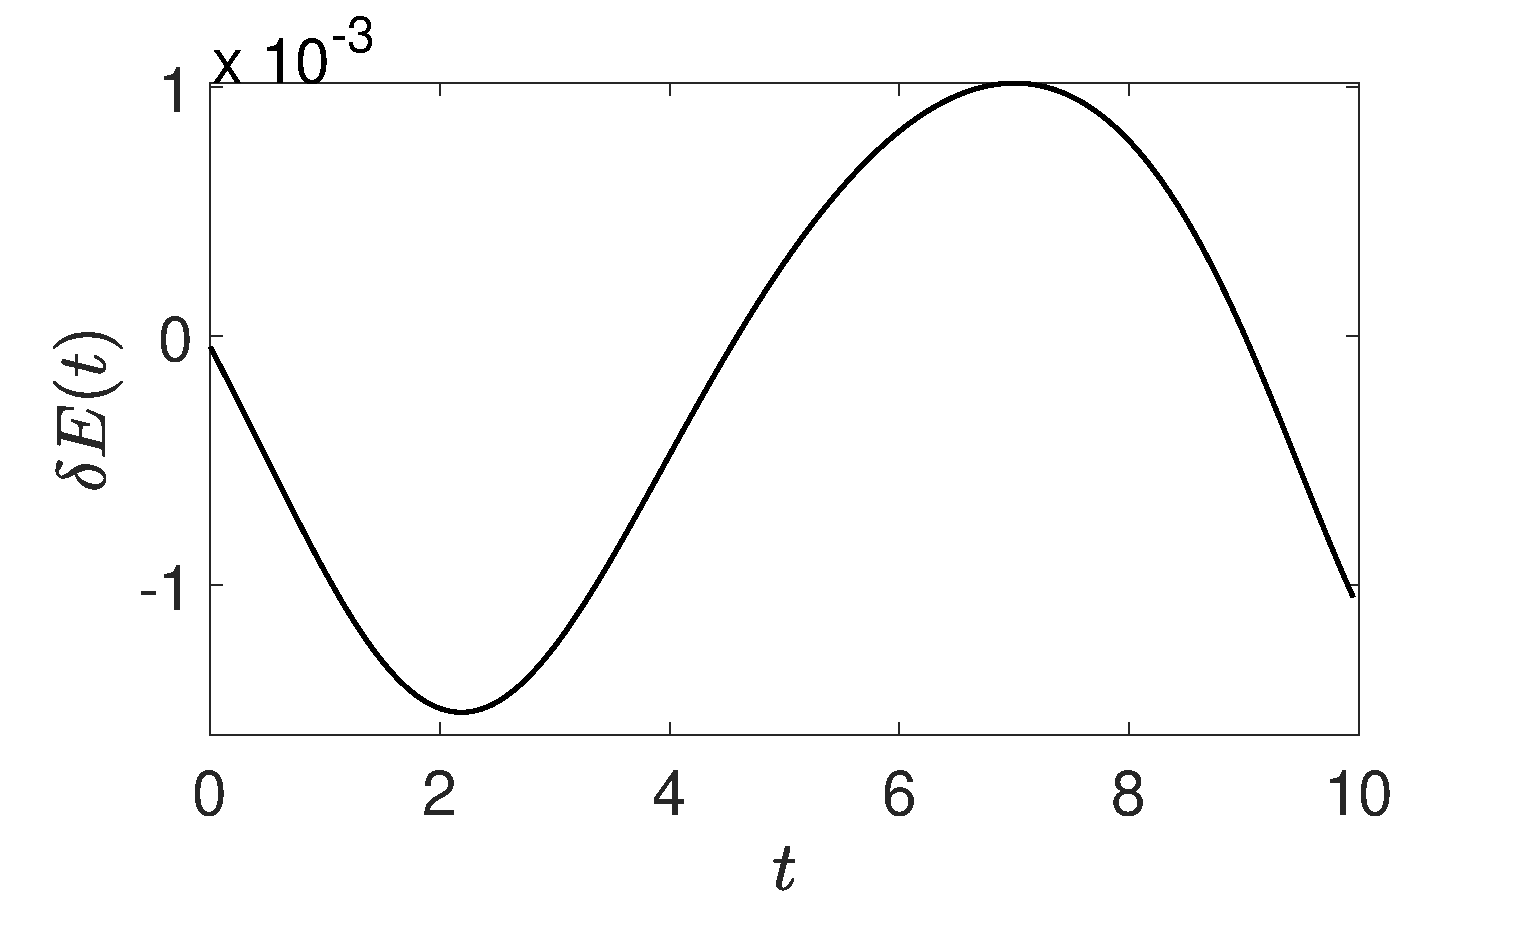
\includegraphics[width=8cm,height=6cm]{energy_wm_1_modu_pt6} & 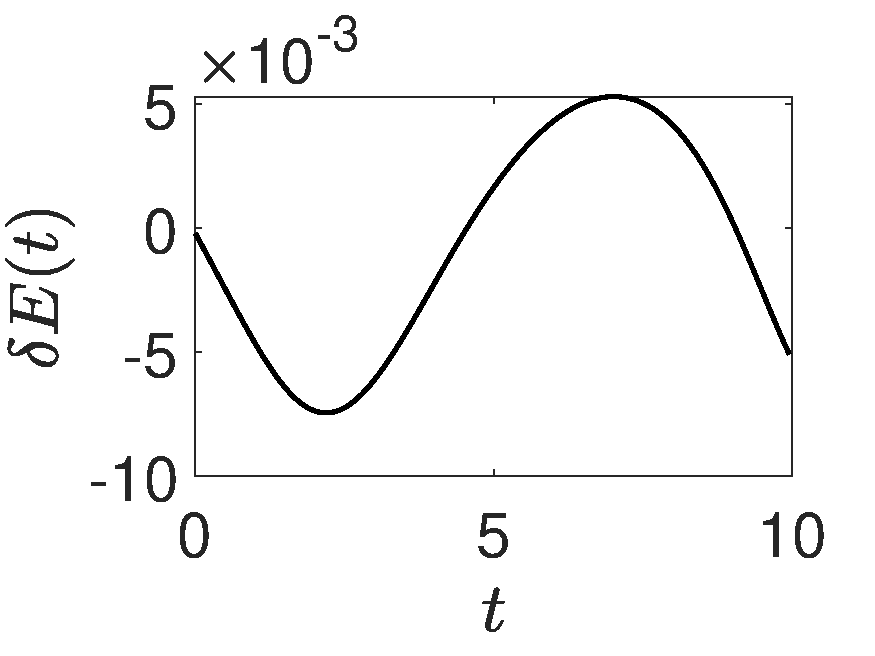
\includegraphics[width=8cm,height=6cm]{energy_wm_5_modu_pt6} \\
(a) $F=.01$ & (b) $F=.05$\\
 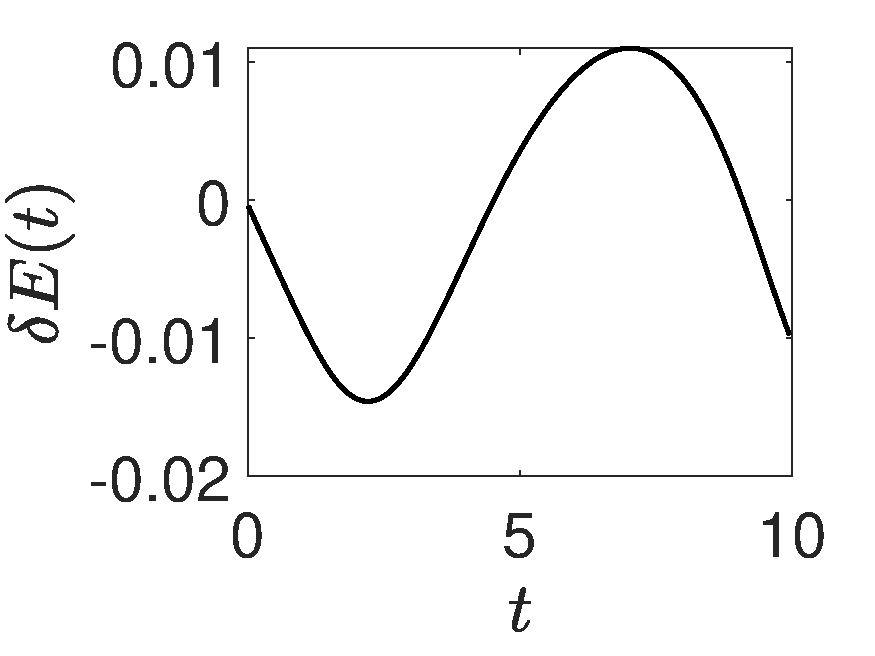
\includegraphics[width=8cm,height=6cm]{energy_wm_10_modu_pt6}\\
 (c) $F=.1$
\end{tabular}
\caption{The relative energy change $\delta E(t)$ for $F=.01$ (a), $F=.05$ (b), and $F=.1$ (c) for $\tilde{m}=.6$ and $\kappa = .43$.  In the relatively moderate nonlinearity case, the increasing Froude number leads to a greater than ten-fold increase in the peak amplitude of the relative energy input.  However presence of greater nonlinearity in the surface wave reduces the overall impact of the patch at the surface as reflected in the overall lower energy difference magnitudes as compared to those in Figure \ref{fig:lowsolenergy}.}
\label{fig:midsolenergy}
\end{figure}

However, in contrast to the $\tilde{m}=.3$ case above, we see that the response of the relative energy input $\delta E(t;F)$ is far more linear in nature, with peaks and troughs being enhanced about equally with rising values of $F$.  We also see that the center of the patch is displaced at a far greater distance relative to its starting position, showing the greater impact of the higher amplitude, faster moving surface wave.  
%%%%%%%%%%%%%%%%%%%%%%%%%%%%%%%%%%%%%%%%%%%%%%%%%%%%%%%%%%%%%%%%%%%%%%%%%%%%%%%%%%%
\subsection*{Elliptic Modulus $\tilde{m}=.9$}
Taking $\tilde{m}=.9$, we find that $\kappa = .35$, this corresponds to $M \approx 7.4$.  Taking $K_{T}=512$, this gives $\delta x = .029$.  The unscaled amplitude of the cnoidal initial conditions is given by $8(\tilde{m}\kappa)^{2}\approx .8$.  Thus, somewhat suprisingly, we could use the largest amplitude wave when the initial condition was closest to that of a solitary wave profile.  Likewise, aside from causing a slight broadening and thus decrease in maximum amplitude of the near solitary wave, vorticity has the least relative impact on the wave.  Thus, if we treat the $\tilde{m}=.9$ as the `most' nonlinear of the three cases examined, since this corresponds to the case closest to that of a nonlinear solitary wave, we see vorticity has the least overall impact on the most nonlinear of waves.  
\begin{figure}
\centering
\begin{tabular}{cc}
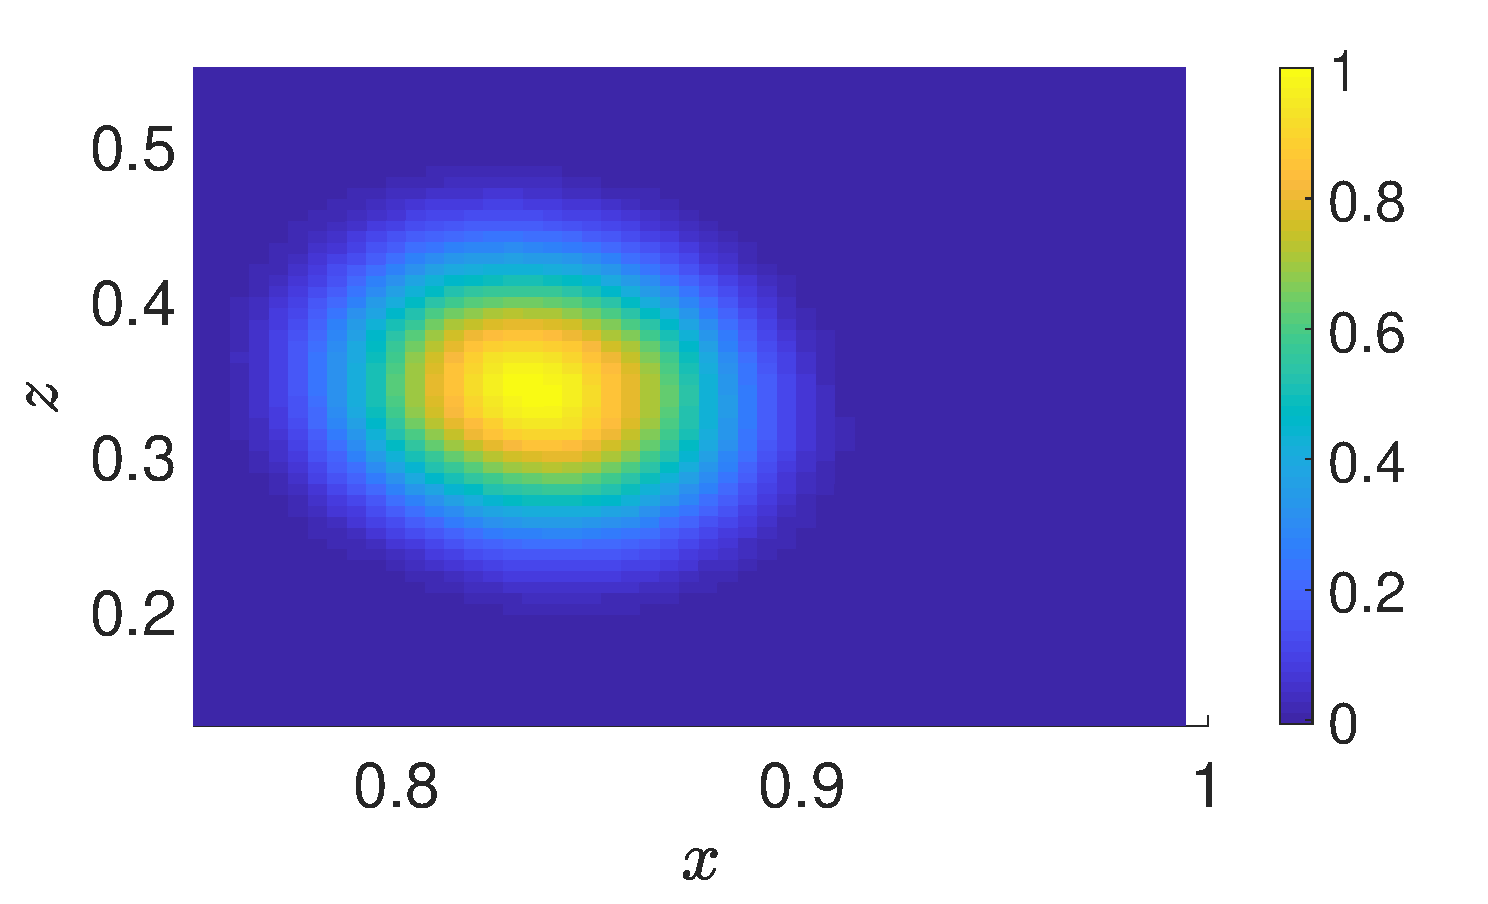
\includegraphics[width=.45\textwidth]{vorticity_wm_1_modu_pt9} & 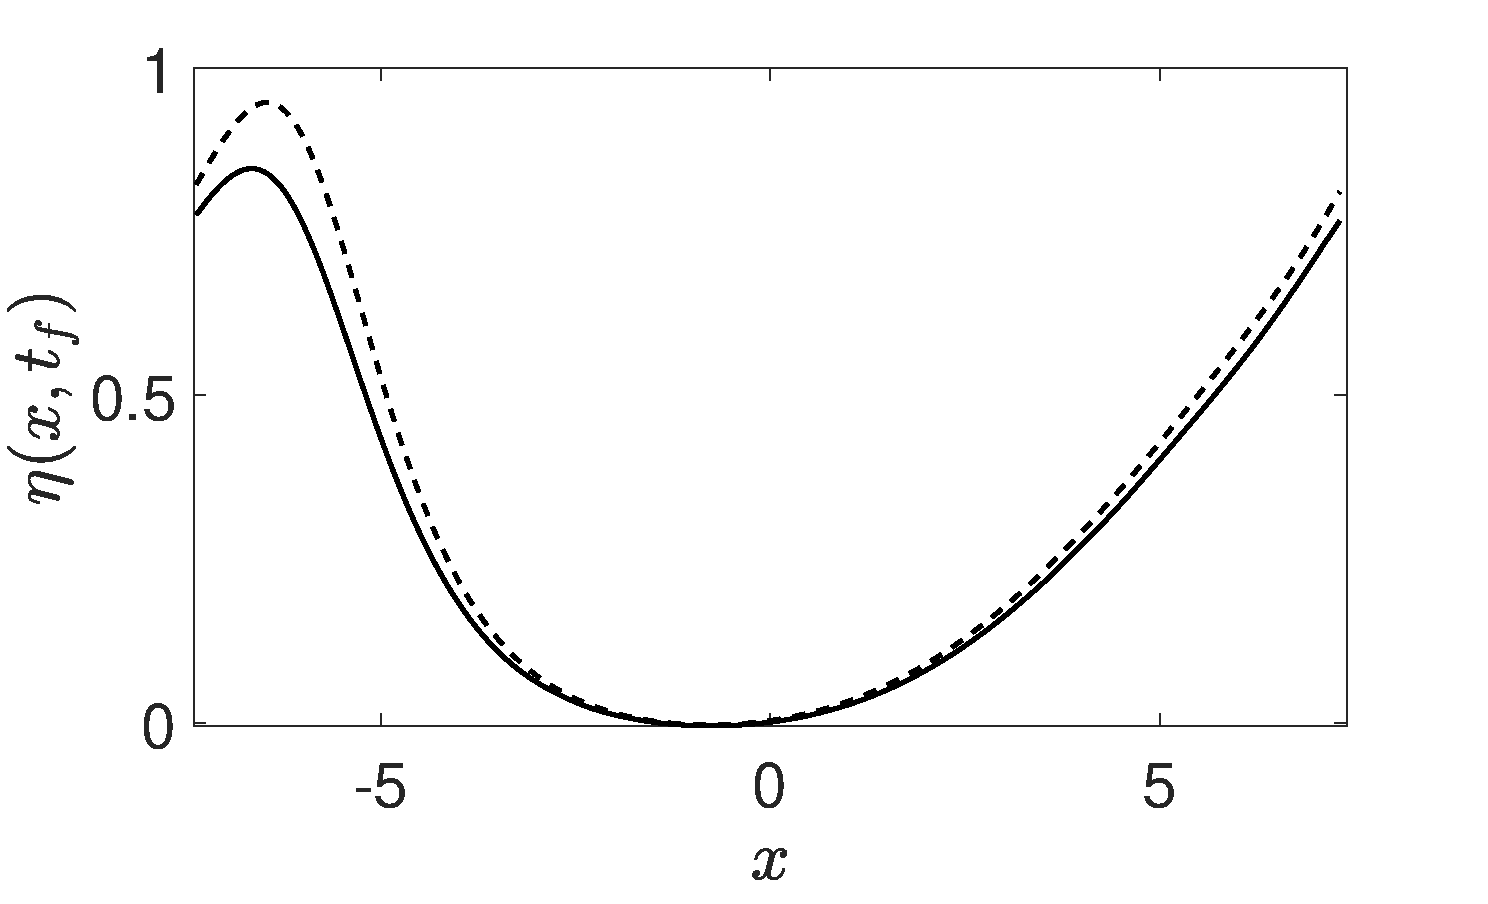
\includegraphics[width=.45\textwidth]{profiles_wm_1_modu_pt9}\\
(a)  $F=.01$ & (b)  $F=.01$\\
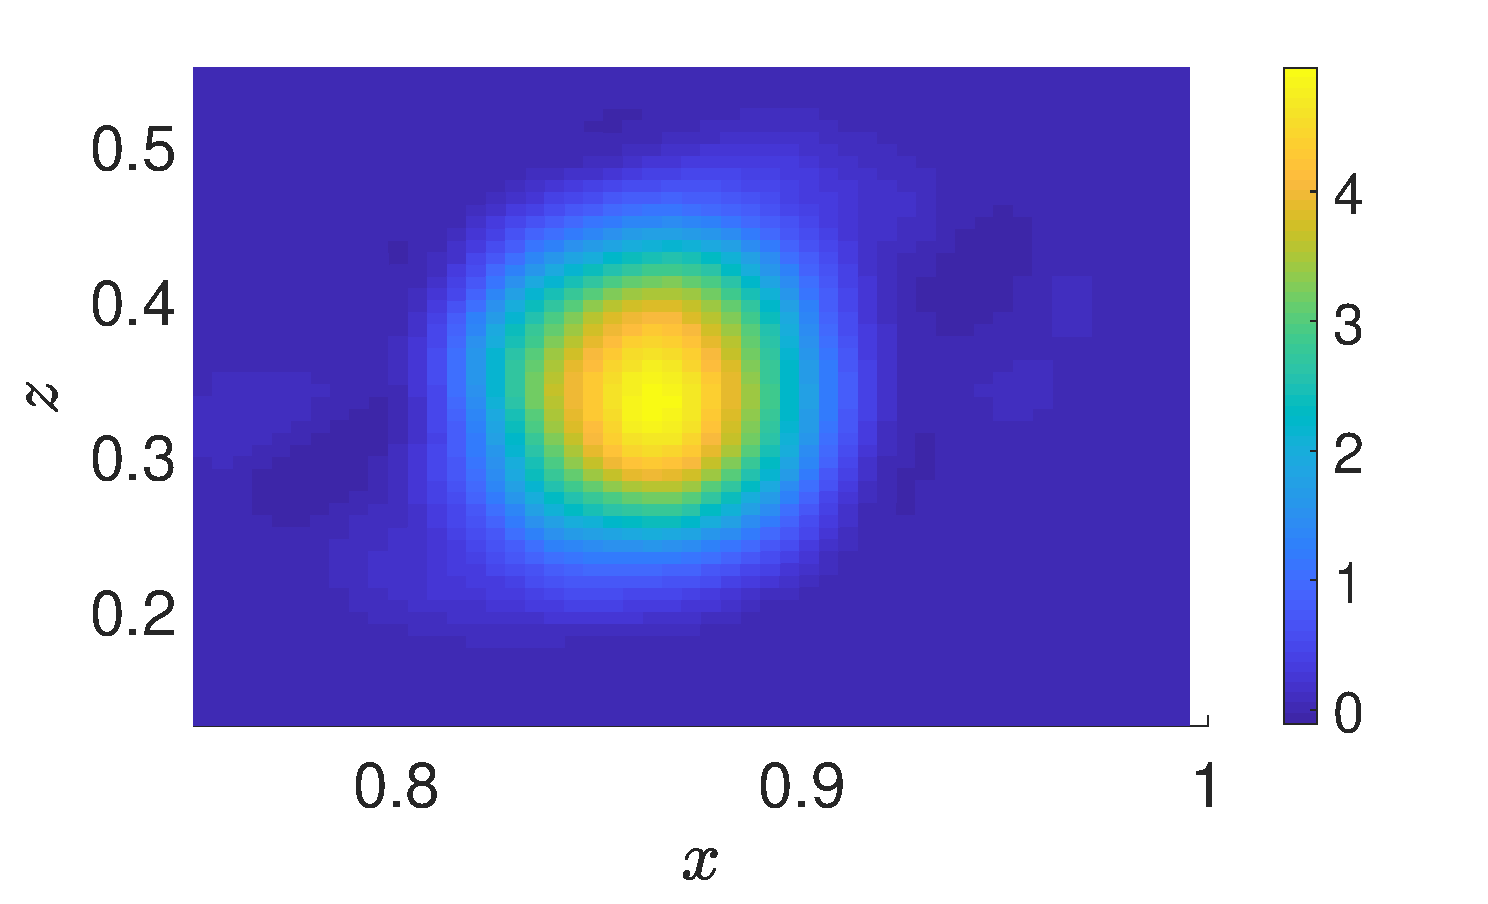
\includegraphics[width=.45\textwidth]{vorticity_wm_5_modu_pt9} & 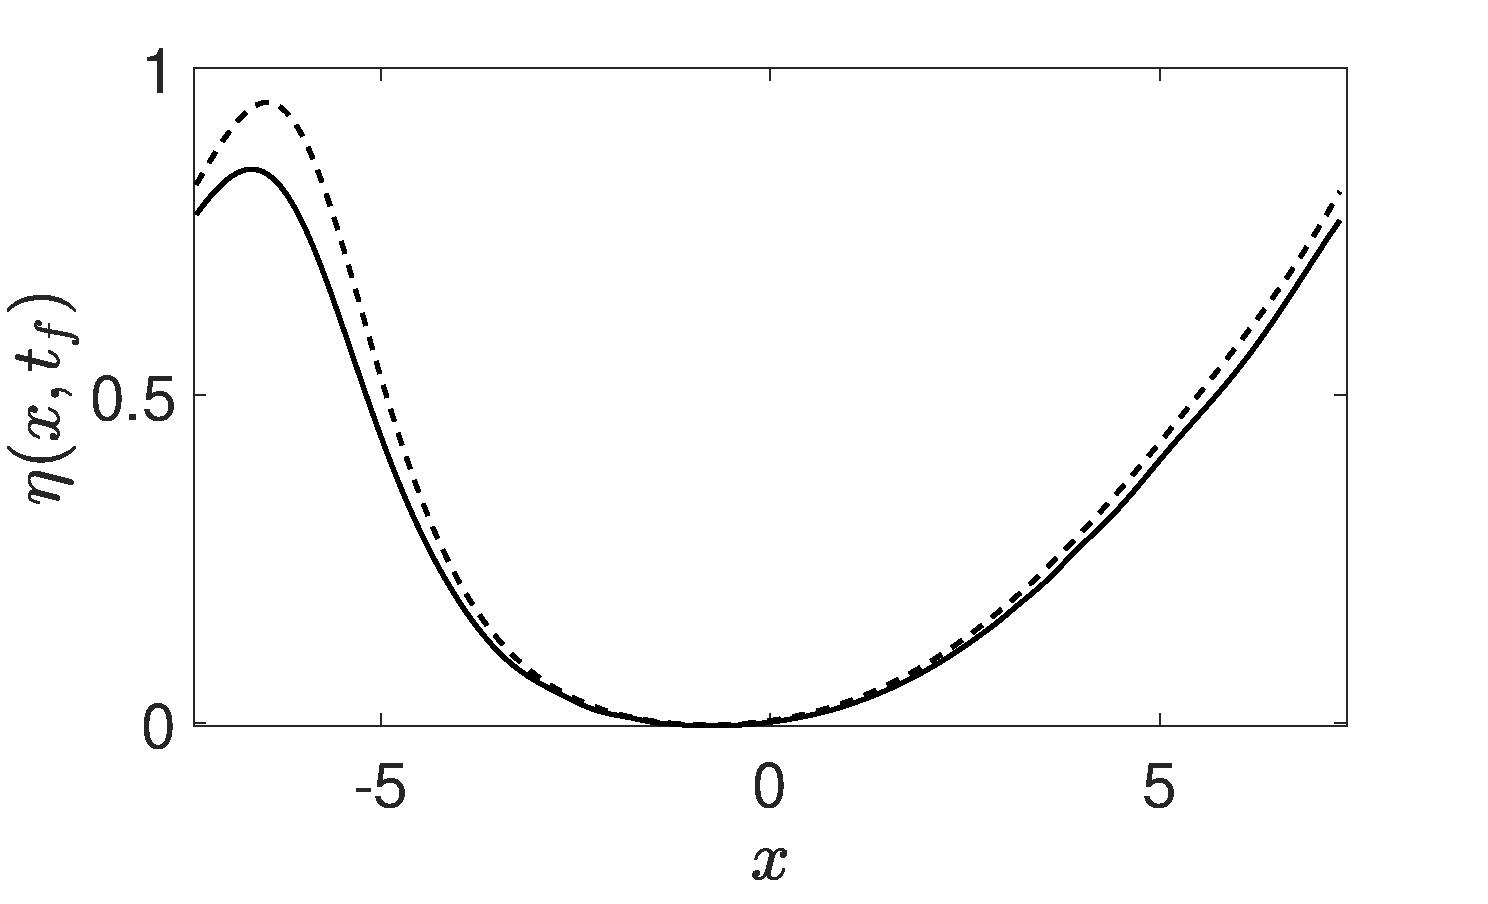
\includegraphics[width=.45\textwidth]{profiles_wm_5_modu_pt9}\\
(c)  $F=.05$ & (d)  $F=.05$\\
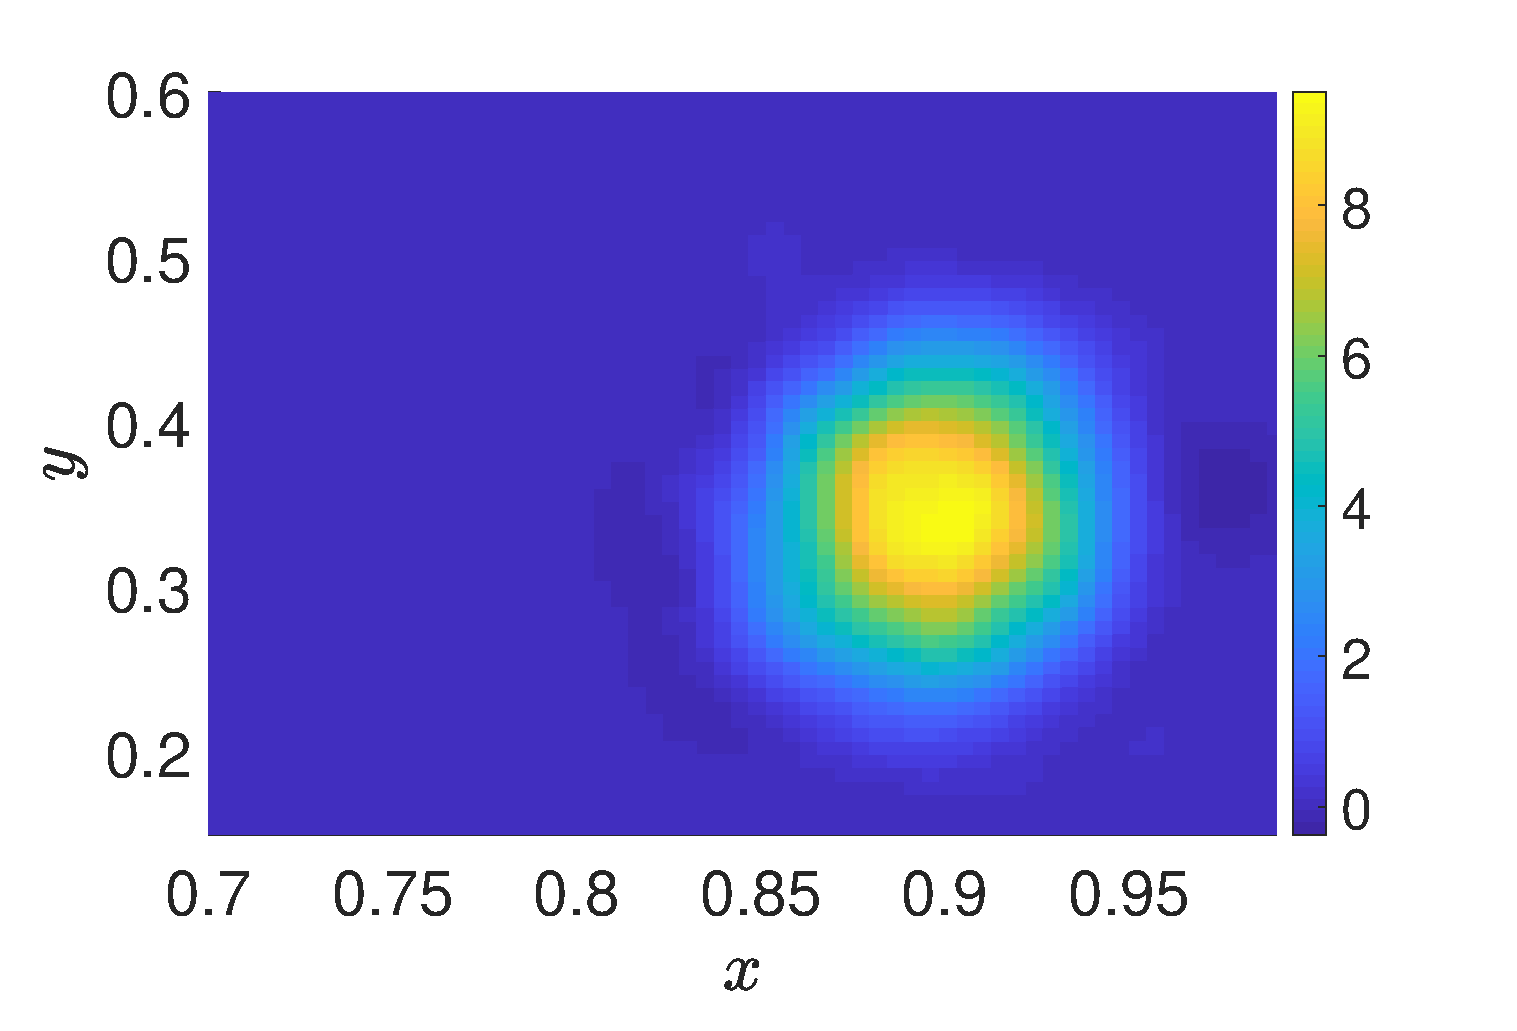
\includegraphics[width=.45\textwidth]{vorticity_wm_10_modu_pt9} & 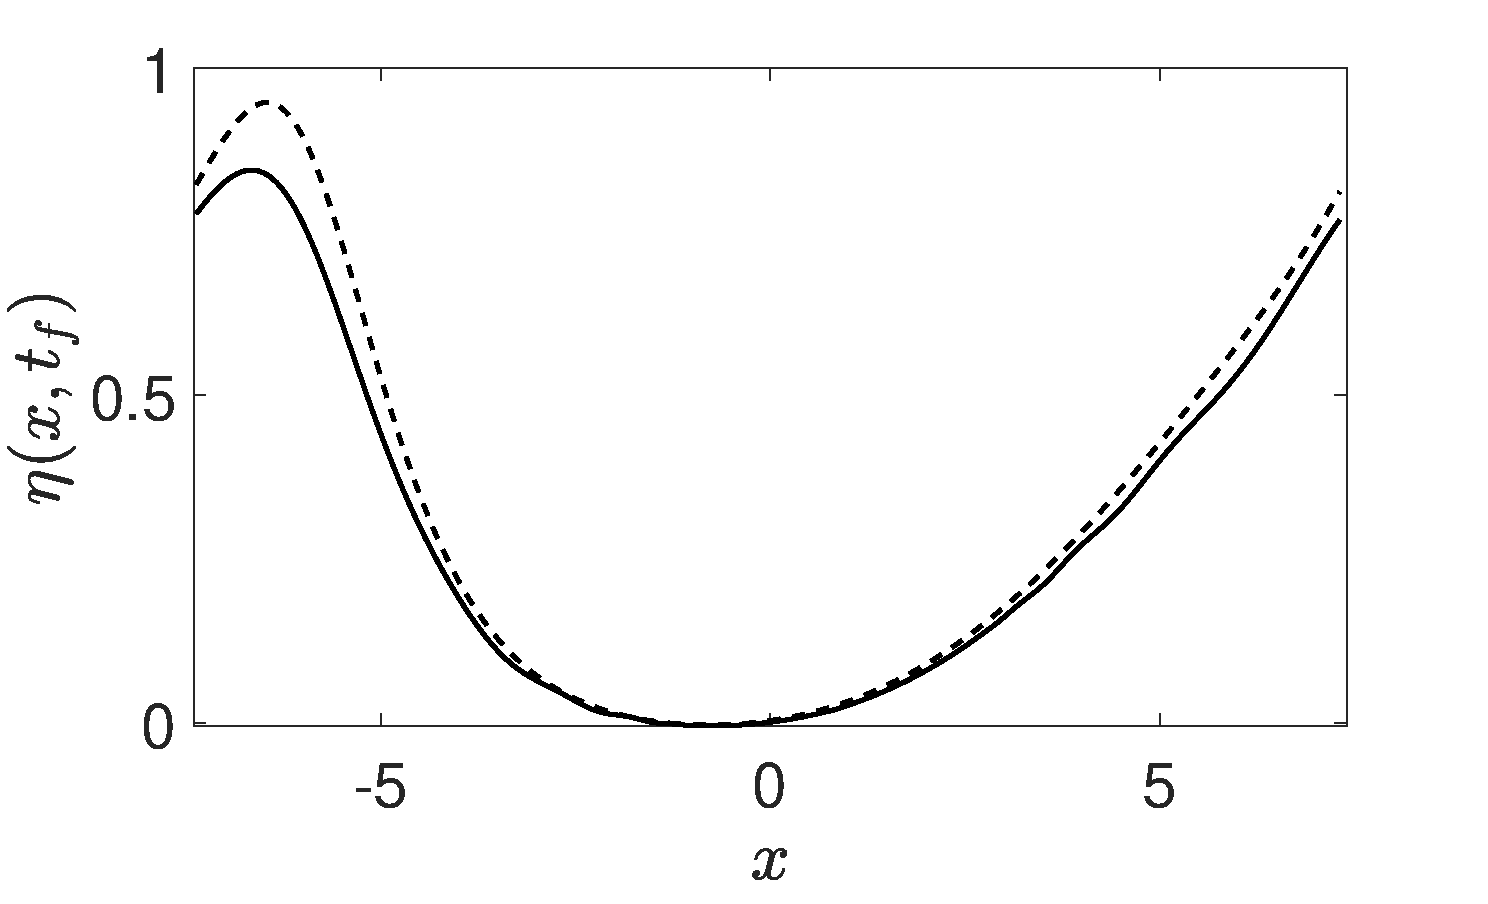
\includegraphics[width=.45\textwidth]{profiles_wm_10_modu_pt9}\\
(e)  $F=.1$ & (f)  $F=.1$
\end{tabular}
\caption{The vortex patches are shown on the left for various values of Froude number $F$, while comparisons of a cnoidal wave over a vortex patch(-) to a cnoidal wave over an irrotational fluid (--) are shown on the right.  Relative to the initial horizontal displacement of $x_{c}=0$, the center of the patch is now between $.8$ and $.9$.  Here $\mu=.2$, $\gamma=\sqrt{\mu}$, $t_{f}=2/\mu$, $\tilde{m}=.9$, $\kappa = .35$.}
\label{fig:highsolwave}
\end{figure}

\begin{figure}
\centering
\begin{tabular}{cc}
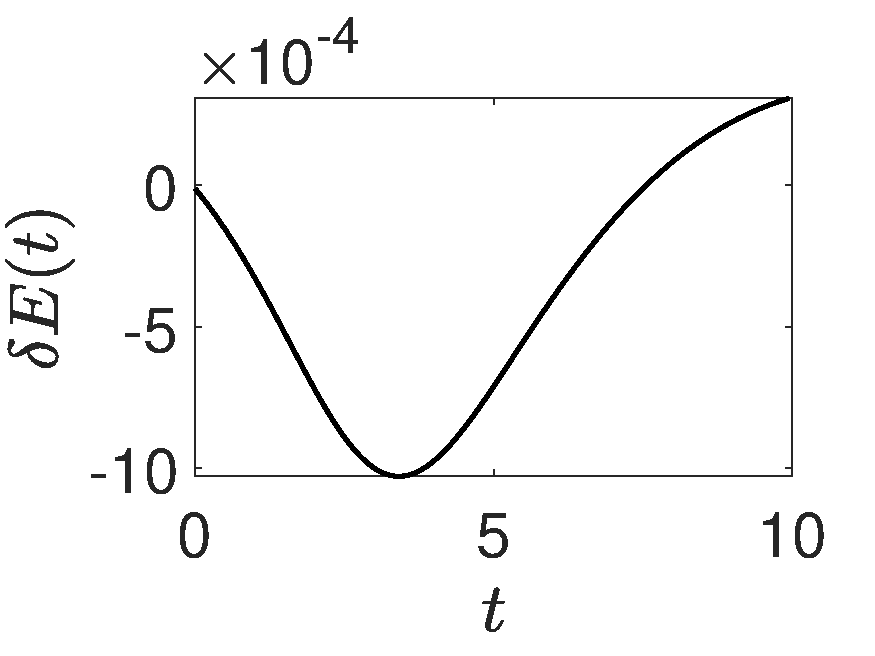
\includegraphics[width=8cm,height=6cm]{energy_wm_1_modu_pt9} & 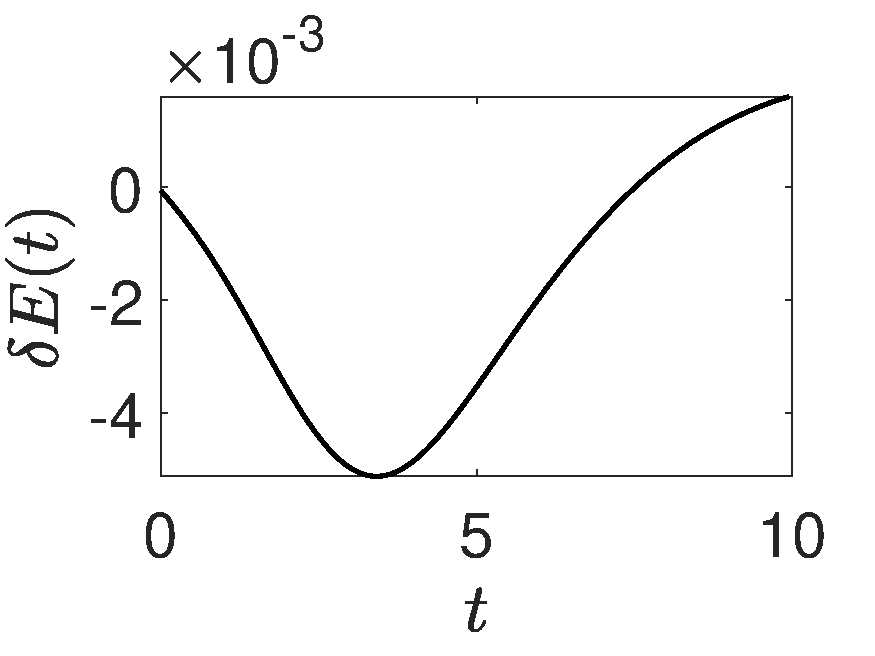
\includegraphics[width=8cm,height=6cm]{energy_wm_5_modu_pt9} \\
(a) $F=.01$ & (b) $F=.05$\\
 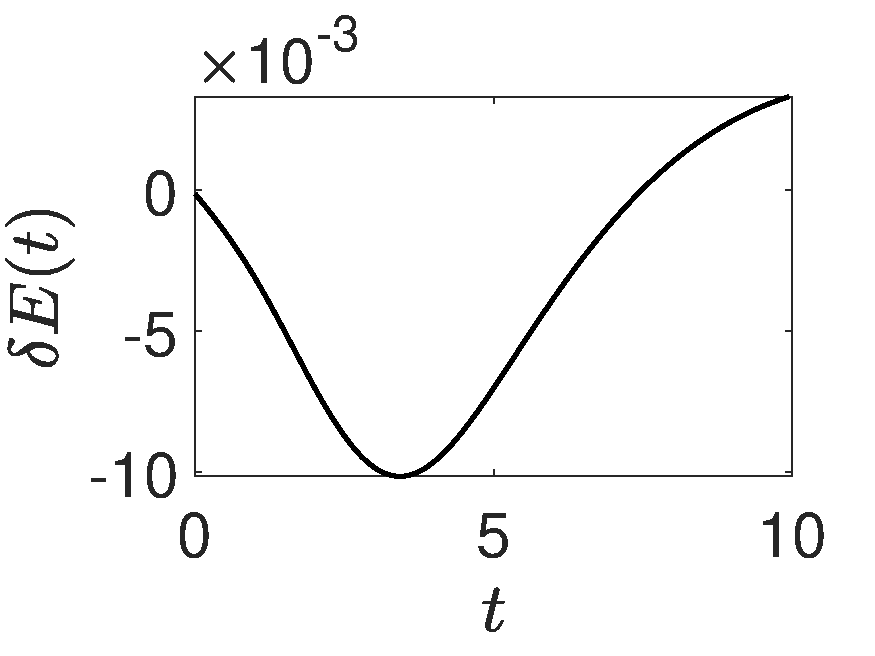
\includegraphics[width=8cm,height=6cm]{energy_wm_10_modu_pt9}\\
 (c) $F=.1$
\end{tabular}
\caption{The relative energy change $\delta E(t)$ for $F=.01$ (a), $F=.05$ (b), and $F=.1$ (c) for $\tilde{m}=.9$ and $\kappa = .35$.  In the relatively strong nonlinearity case, the increasing Froude number leads to a greater than ten-fold loss of the relative energy change in the surface.  However the  presence of greater nonlinearity in the surface wave reduces the overall impact of the patch at the surface as reflected in the overall lower energy difference magnitudes as compared to those in Figure \ref{fig:lowsolenergy}.}
\label{fig:highsolenergy}
\end{figure}

This is especially seen by the weak response of $\delta E(t;F)$ plotted in Figure \ref{fig:highsolwave}.  We also get the clearest correlation between the loss in amplitude seen in Figure \ref{fig:highsolwave} and the relative energy input, which is largely negative though stretched out over a longer time scale than in comparison to the energy dynamics seen above.   We also see that the center of the patch is displaced at a the greatest distance relative to its starting position, showing the strong effect that relatively large amplitude, fast moving nonlinear waves have on the patch.  We see from the energy dynamics that a likely explanation of this enhanced transport is that the patch is able to pull energy from the more nonlinear surface wave.  
%%%%%%%%%%%%%%%%%%%%%%%%%%%%%%%%%%%%%%%%%%%%%%%%%%%%%%%%%%%%%%%%%%%%%%%%%%%%%%%%%%%
%%%%%%%%%%%%%%%%%%%%%%%%%%%%%%%%%%%%%%%%%%%%%%%%%%%%%%%%%%%%%%%%%%%%%%%%%%%%%%%%%%%
\section{Conclusion}
We have in this paper provided detailed numerical simulations of a vortex patch under a free-surface wave.  This was done by bringing together approaches from both the nonlinear ocean waves and larger computational fluid dynamics community.  Via our simulations, we have shown how vortex patches induce non-trivial deformations of propagating nonlinear waves coming from the shallow-water, KdV limit.  The deformations are especially significant when the waves are low amplitude, essentially linear modes.  Our simulations allow for greater quantitative insight by tracking the relative energy transfer of the patch to the wave, the dynamics and features of which we show correlates strongly to the presence or absence of significant deformations in the surface wave due to the vortex patch.  

\section*{Acknowledgements}

\section*{Appendix}
We here provide details about the Dirichlet-to-Neumann Operator (DNO) for the sake of completeness; see \cite{craig,guyenne} for greater details.    The DNO $G(\eta)$ in the shallow-water scalings used throughout the body of the paper is found via expading in powers of $\eta$ so that the kinematic condition becomes 
\[
\eta_{t} - \frac{1}{\gamma}P_{v}(x,1+\mu \eta,t) = \left(G_{0} + \mu G_{1} + \mu^{2}  G_{2} + \cdots \right)Q.
\]
Defining the Fourier transform of a periodic function $f(x)$ to be $\hat{f}$, so that 
\[
\hat{f}(k) = \frac{1}{2}\int_{-M}^{M}f(x)e^{-i\pi k x} dx, ~ k\in \mathbb{Z},
\]
we define, for a linear operator $L$, its associated symbol $\hat{L}(k)$ by way of the formula 
\[
\hat{L}(k)\hat{f}(k) = \frac{1}{2M}\int_{-M}^{M} Lf(x) e^{-i\pi k x/M}dx.
\]
We then get 
\[
\hat{G}_{0}(k) = -\frac{i}{\gamma}\tanh(\pi \gamma k),
\]
and, for $m\geq 1$, 
\begin{align*}
G_{m}Q = & -\sum_{j=1}^{\lfloor{m/2}\rfloor}\frac{1}{(2j)!}D^{2j}_{\gamma}\left(\eta^{2j}G_{m-2j}Q\right) \\
& - \gamma^{2}\p_{x}G_{0} \sum_{j=0}^{\lfloor{(m-1)/2}\rfloor}\frac{D_{\gamma}^{2j}}{(2j+1)!}\left(\eta^{2j+1}G_{m-2j-1}Q\right) - \frac{1}{m!}L_{m} \p_{x}D_{\gamma}^{m-1}\left(\eta^{m}Q \right),
\end{align*}
where
\[
\hat{D}_{\gamma} = \pi \gamma k,
\]
and
\[
\hat{L}_{m} = \left\{
\ba{rl}
1,  & m~\mbox{is odd}, \\
i\gamma \hat{G}_{0}(k),  & m~\mbox{is even}.
\ea
\right.
\]
This recursive formula is readily computable, and for the shallow-water scalings we pick, achieving machine-precision is relatively straightforward.  
\bibliography{waves_over_vortices}
\bibliographystyle{unsrt}
\end{document}